% -*- coding: utf-8 -*-
%!TEX program = xelatex
\ifx \allfiles \undefined
\documentclass[12pt]{ctexbook}%draft,
%\usepackage{xeCJK}
%\usepackage[14pt]{extsizes} %支持8,9,10,11,12,14,17,20pt

%===================文档页面设置====================
%---------------------印刷版尺寸--------------------
%\usepackage[a4paper,hmargin={2.3cm,1.7cm},vmargin=2.3cm,driver=xetex]{geometry}
%--------------------电子版------------------------
\usepackage[a4paper,margin=2cm,driver=xetex]{geometry}
%\usepackage[paperwidth=9.2cm, paperheight=12.4cm, width=9cm, height=12cm,top=0.2cm,
%            bottom=0.4cm,left=0.2cm,right=0.2cm,foot=0cm, nohead,nofoot,driver=xetex]{geometry}

%===================自定义颜色=====================
\usepackage{xcolor}
  \definecolor{mybackgroundcolor}{cmyk}{0.03,0.03,0.18,0}
  \definecolor{myblue}{rgb}{0,0.2,0.6}

%====================字体设置======================
%--------------------中文字体----------------------
%-----------------------xeCJK下设置中文字体------------------------------%
\setCJKfamilyfont{song}{SimSun}                             %宋体 song
\newcommand{\song}{\CJKfamily{song}}                        % 宋体   (Windows自带simsun.ttf)
\setCJKfamilyfont{xs}{NSimSun}                              %新宋体 xs
\newcommand{\xs}{\CJKfamily{xs}}
\setCJKfamilyfont{fs}{FangSong_GB2312}                      %仿宋2312 fs
\newcommand{\fs}{\CJKfamily{fs}}                            %仿宋体 (Windows自带simfs.ttf)
\setCJKfamilyfont{kai}{KaiTi_GB2312}                        %楷体2312  kai
\newcommand{\kai}{\CJKfamily{kai}}
\setCJKfamilyfont{yh}{Microsoft YaHei}                    %微软雅黑 yh
\newcommand{\yh}{\CJKfamily{yh}}
\setCJKfamilyfont{hei}{SimHei}                                    %黑体  hei
\newcommand{\hei}{\CJKfamily{hei}}                          % 黑体   (Windows自带simhei.ttf)
\setCJKfamilyfont{msunicode}{Arial Unicode MS}            %Arial Unicode MS: msunicode
\newcommand{\msunicode}{\CJKfamily{msunicode}}
\setCJKfamilyfont{li}{LiSu}                                            %隶书  li
\newcommand{\li}{\CJKfamily{li}}
\setCJKfamilyfont{yy}{YouYuan}                             %幼圆  yy
\newcommand{\yy}{\CJKfamily{yy}}
\setCJKfamilyfont{xm}{MingLiU}                                        %细明体  xm
\newcommand{\xm}{\CJKfamily{xm}}
\setCJKfamilyfont{xxm}{PMingLiU}                             %新细明体  xxm
\newcommand{\xxm}{\CJKfamily{xxm}}

\setCJKfamilyfont{hwsong}{STSong}                            %华文宋体  hwsong
\newcommand{\hwsong}{\CJKfamily{hwsong}}
\setCJKfamilyfont{hwzs}{STZhongsong}                        %华文中宋  hwzs
\newcommand{\hwzs}{\CJKfamily{hwzs}}
\setCJKfamilyfont{hwfs}{STFangsong}                            %华文仿宋  hwfs
\newcommand{\hwfs}{\CJKfamily{hwfs}}
\setCJKfamilyfont{hwxh}{STXihei}                                %华文细黑  hwxh
\newcommand{\hwxh}{\CJKfamily{hwxh}}
\setCJKfamilyfont{hwl}{STLiti}                                        %华文隶书  hwl
\newcommand{\hwl}{\CJKfamily{hwl}}
\setCJKfamilyfont{hwxw}{STXinwei}                                %华文新魏  hwxw
\newcommand{\hwxw}{\CJKfamily{hwxw}}
\setCJKfamilyfont{hwk}{STKaiti}                                    %华文楷体  hwk
\newcommand{\hwk}{\CJKfamily{hwk}}
\setCJKfamilyfont{hwxk}{STXingkai}                            %华文行楷  hwxk
\newcommand{\hwxk}{\CJKfamily{hwxk}}
\setCJKfamilyfont{hwcy}{STCaiyun}                                 %华文彩云 hwcy
\newcommand{\hwcy}{\CJKfamily{hwcy}}
\setCJKfamilyfont{hwhp}{STHupo}                                 %华文琥珀   hwhp
\newcommand{\hwhp}{\CJKfamily{hwhp}}

\setCJKfamilyfont{fzsong}{Simsun (Founder Extended)}     %方正宋体超大字符集   fzsong
\newcommand{\fzsong}{\CJKfamily{fzsong}}
\setCJKfamilyfont{fzyao}{FZYaoTi}                                    %方正姚体  fzy
\newcommand{\fzyao}{\CJKfamily{fzyao}}
\setCJKfamilyfont{fzshu}{FZShuTi}                                    %方正舒体 fzshu
\newcommand{\fzshu}{\CJKfamily{fzshu}}

\setCJKfamilyfont{asong}{Adobe Song Std}                        %Adobe 宋体  asong
\newcommand{\asong}{\CJKfamily{asong}}
\setCJKfamilyfont{ahei}{Adobe Heiti Std}                            %Adobe 黑体  ahei
\newcommand{\ahei}{\CJKfamily{ahei}}
\setCJKfamilyfont{akai}{Adobe Kaiti Std}                            %Adobe 楷体  akai
\newcommand{\akai}{\CJKfamily{akai}}

%------------------------------设置字体大小------------------------%
\newcommand{\chuhao}{\fontsize{42pt}{\baselineskip}\selectfont}     %初号
\newcommand{\xiaochuhao}{\fontsize{36pt}{\baselineskip}\selectfont} %小初号
\newcommand{\yihao}{\fontsize{28pt}{\baselineskip}\selectfont}      %一号
\newcommand{\xiaoyihao}{\fontsize{24pt}{\baselineskip}\selectfont}
\newcommand{\erhao}{\fontsize{21pt}{\baselineskip}\selectfont}      %二号
\newcommand{\xiaoerhao}{\fontsize{18pt}{\baselineskip}\selectfont}  %小二号
\newcommand{\sanhao}{\fontsize{15.75pt}{\baselineskip}\selectfont}  %三号
\newcommand{\sihao}{\fontsize{14pt}{\baselineskip}\selectfont}%     四号
\newcommand{\xiaosihao}{\fontsize{12pt}{\baselineskip}\selectfont}  %小四号
\newcommand{\wuhao}{\fontsize{10.5pt}{\baselineskip}\selectfont}    %五号
\newcommand{\xiaowuhao}{\fontsize{9pt}{\baselineskip}\selectfont}   %小五号
\newcommand{\liuhao}{\fontsize{7.875pt}{\baselineskip}\selectfont}  %六号
\newcommand{\qihao}{\fontsize{5.25pt}{\baselineskip}\selectfont}    %七号   %中文字体及字号设置
\xeCJKDeclareSubCJKBlock{SIP}{
  "20000 -> "2A6DF,   % CJK Unified Ideographs Extension B
  "2A700 -> "2B73F,   % CJK Unified Ideographs Extension C
  "2B740 -> "2B81F    % CJK Unified Ideographs Extension D
}
%\setCJKmainfont[SIP={[AutoFakeBold=1.8,Color=red]Sun-ExtB},BoldFont=黑体]{宋体}    % 衬线字体 缺省中文字体

\setCJKmainfont{simsun.ttc}[
  Path=fonts/,
  SIP={[Path=fonts/,AutoFakeBold=1.8,Color=red]simsunb.ttf},
  BoldFont=simhei.ttf
]

%SimSun-ExtB
%Sun-ExtB
%AutoFakeBold:自动伪粗,即正文使用\bfseries时生僻字使用伪粗体;
%FakeBold:强制伪粗,即正文中生僻字均使用伪粗体
%\setCJKmainfont[BoldFont=STHeiti,ItalicFont=STKaiti]{STSong}
%\setCJKsansfont{微软雅黑}黑体
%\setCJKsansfont[BoldFont=STHeiti]{STXihei} %serif是有衬线字体sans serif 无衬线字体
%\setCJKmonofont{STFangsong}    %中文等宽字体

%--------------------英文字体----------------------
\setmainfont{simsun.ttc}[
  Path=fonts/,
  BoldFont=simhei.ttf
]
%\setmainfont[BoldFont=黑体]{宋体}  %缺省英文字体
%\setsansfont
%\setmonofont

%===================目录分栏设置====================
\usepackage[toc,lof,lot]{multitoc}    % 目录(含目录、表格目录、插图目录)分栏设置
  %\renewcommand*{\multicolumntoc}{3} % toc分栏数设置,默认为两栏(\multicolumnlof,\multicolumnlot)
  %\setlength{\columnsep}{1.5cm}      % 调整分栏间距
  \setlength{\columnseprule}{0.2pt}   % 调整分栏竖线的宽度

%==================章节格式设置====================
\setcounter{secnumdepth}{3} % 章节等编号深度 3:子子节\subsubsection
\setcounter{tocdepth}{2}    % 目录显示等度 2:子节

\xeCJKsetup{%
  CJKecglue=\hspace{0.15em},      % 调整中英(含数字)间的字间距
  %CJKmath=true,                  % 在数学环境中直接输出汉字(不需要\text{})
  AllowBreakBetweenPuncts=true,   % 允许标点中间断行,减少文字行溢出
}

\ctexset{%
  part={
    name={,篇},
    number=\SZX{part},
    format={\chuhao\bfseries\centering},
    nameformat={},titleformat={}
  },
  section={
    number={\chinese{section}},
    name={第,节}
  },
  subsection={
    number={\chinese{subsection}、},
    aftername={\hspace{-0.01em}}
  },
  subsubsection={
    number={(\chinese{subsubsection})},
    aftername={\hspace {-0.01em}},
    beforeskip={1.3ex minus .8ex},
    afterskip={1ex minus .6ex},
    indent={\parindent}
  },
  paragraph={
    beforeskip=.1\baselineskip,
    indent={\parindent}
  }
}

\newcommand*\SZX[1]{%
  \ifcase\value{#1}%
    \or 上%
    \or 中%
    \or 下%
  \fi
}

%====================页眉设置======================
\usepackage{titleps}%或者\usepackage{titlesec},titlesec包含titleps
\newpagestyle{special}[\small\sffamily]{
  %\setheadrule{.1pt}
  \headrule
  \sethead[\usepage][][\chaptertitle]
  {\chaptertitle}{}{\usepage}
}

\newpagestyle{main}[\small\sffamily]{
  \headrule
  %\sethead[\usepage][][第\thechapter 章\quad\chaptertitle]
%  {\thesection\quad\sectiontitle}{}{\usepage}}
  \sethead[\usepage][][第\chinese{chapter}章\quad\chaptertitle]
  {第\chinese{section}节\quad\sectiontitle}{}{\usepage}
}

\newpagestyle{main2}[\small\sffamily]{
  \headrule
  \sethead[\usepage][][第\chinese{chapter}章\quad\chaptertitle]
  {第\chinese{section}節\quad\sectiontitle}{}{\usepage}
}

%================ PDF 书签设置=====================
\usepackage{bookmark}[
  depth=2,        % 书签深度 2:子节
  open,           % 默认展开书签
  openlevel=2,    % 展开书签深度 2:子节
  numbered,       % 显示编号
  atend,
]
  % 相比hyperref,bookmark宏包大多数时候只需要编译一次,
  % 而且书签的颜色和字体也可以定制。
  % 比hyperref 更专业 (自动加载hyperref)

%\bookmarksetup{italic,bold,color=blue} % 书签字体斜体/粗体/颜色设置

%------------重置每篇章计数器,必须在hyperref/bookmark之后------------
\makeatletter
  \@addtoreset{chapter}{part}
\makeatother

%------------hyperref 超链接设置------------------------
\hypersetup{%
  pdfencoding=auto,   % 解决新版ctex,引起hyperref UTF-16预警
  colorlinks=true,    % 注释掉此项则交叉引用为彩色边框true/false
  pdfborder=001,      % 注释掉此项则交叉引用为彩色边框
  citecolor=teal,
  linkcolor=myblue,
  urlcolor=black,
  %psdextra,          % 配合使用bookmark宏包,可以直接在pdf 书签中显示数学公式
}

%------------PDF 属性设置------------------------------
\hypersetup{%
  pdfkeywords={黄帝内经,内经,内经讲义,21世纪课程教材},    % 关键词
  %pdfsubject={latex},        % 主题
  pdfauthor={主编:王洪图},   % 作者
  pdftitle={内经讲义},        % 标题
  %pdfcreator={texlive2011}   % pdf创建器
}

%------------PDF 加密----------------------------------
%仅适用于xelatex引擎 基于xdvipdfmx
%\special{pdf:encrypt ownerpw (abc) userpw (xyz) length 128 perm 2052}

%仅适用于pdflatex引擎
%\usepackage[owner=Donald,user=Knuth,print=false]{pdfcrypt}

%其他可使用第三方工具 如:pdftk
%pdftk inputfile.pdf output outputfile.pdf encrypt_128bit owner_pw yourownerpw user_pw youruserpw

%=============自定义环境、列表及列表设置================
% 标题
\def\biaoti#1{\vspace{1.7ex plus 3ex minus .2ex}{\bfseries #1}}%\noindent\hei
% 小标题
\def\xiaobt#1{{\bfseries #1}}
% 小结
\def\xiaojie {\vspace{1.8ex plus .3ex minus .3ex}\centerline{\large\bfseries 小\ \ 结}\vspace{.1\baselineskip}}
% 作者
\def\zuozhe#1{\rightline{\bfseries #1}}

\newcounter{yuanwen}    % 新计数器 yuanwen
\newcounter{jiaozhu}    % 新计数器 jiaozhu

\newenvironment{yuanwen}[2][【原文】]{%
  %\biaoti{#1}\par
  \stepcounter{yuanwen}   % 计数器 yuanwen+1
  \bfseries #2}
  {}

\usepackage{enumitem}
\newenvironment{jiaozhu}[1][【校注】]{%
  %\biaoti{#1}\par
  \stepcounter{jiaozhu}   % 计数器 jiaozhu+1
  \begin{enumerate}[%
    label=\mylabel{\arabic*}{\circledctr*},before=\small,fullwidth,%
    itemindent=\parindent,listparindent=\parindent,%labelsep=-1pt,%labelwidth=0em,
    itemsep=0pt,topsep=0pt,partopsep=0pt,parsep=0pt
  ]}
  {\end{enumerate}}

%===================注解与原文相互跳转====================
%----------------第1部分 设置相互跳转锚点-----------------
\makeatletter
  \protected\def\mylabel#1#2{% 注解-->原文
    \hyperlink{back:\theyuanwen:#1}{\Hy@raisedlink{\hypertarget{\thejiaozhu:#1}{}}#2}}

  \protected\def\myref#1#2{% 原文-->注解
    \hyperlink{\theyuanwen:#1}{\Hy@raisedlink{\hypertarget{back:\theyuanwen:#1}{}}#2}}
  %此处\theyuanwen:#1实际指thejiaozhu:#1,只是\thejiaozhu计数器还没更新,故使用\theyuanwen计数器代替
\makeatother

\protected\def\myjzref#1{% 脚注中的引用(引用到原文)
  \hyperlink{\theyuanwen:#1}{\circlednum{#1}}}

\def\sb#1{\myref{#1}{\textsuperscript{\circlednum{#1}}}}    % 带圈数字上标

%----------------第2部分 调整锚点垂直距离-----------------
\def\HyperRaiseLinkDefault{.8\baselineskip} %调整锚点垂直距离
%\let\oldhypertarget\hypertarget
%\makeatletter
%  \def\hypertarget#1#2{\Hy@raisedlink{\oldhypertarget{#1}{#2}}}
%\makeatother

%====================带圈数字列表标头====================
\newfontfamily\circledfont[Path = fonts/]{meiryo.ttc}  % 日文字体,明瞭体
%\newfontfamily\circledfont{Meiryo}  % 日文字体,明瞭体

\protected\def\circlednum#1{{\makexeCJKinactive\circledfont\textcircled{#1}}}

\newcommand*\circledctr[1]{%
  \expandafter\circlednum\expandafter{\number\value{#1}}}
\AddEnumerateCounter*\circledctr\circlednum{1}

% 参考自:http://bbs.ctex.org/forum.php?mod=redirect&goto=findpost&ptid=78709&pid=460496&fromuid=40353

%======================插图/tikz图========================
\usepackage{graphicx,subcaption,wrapfig}    % 图,subcaption含子图功能代替subfig,图文混排
  \graphicspath{{img/}}                     % 设置图片文件路径

\def\pgfsysdriver{pgfsys-xetex.def}         % 设置tikz的驱动引擎
\usepackage{tikz}
  \usetikzlibrary{calc,decorations.text,arrows,positioning}

%---------设置tikz图片默认格式(字号、行间距、单元格高度)-------
\let\oldtikzpicture\tikzpicture
\renewcommand{\tikzpicture}{%
  \small
  \renewcommand{\baselinestretch}{0.2}
  \linespread{0.2}
  \oldtikzpicture
}

%=========================表格相关===============================
\usepackage{%
  multirow,                   % 单元格纵向合并
  array,makecell,longtable,   % 表格功能加强,tabu的依赖
  tabu-last-fix,              % "强大的表格工具" 本地修复版
  diagbox,                    % 表头斜线
  threeparttable,             % 表格内脚注(需打补丁支持tabu,longtabu)
}

%----------给threeparttable打补丁用于tabu,longtabu--------------
%解决方案来自:http://bbs.ctex.org/forum.php?mod=redirect&goto=findpost&ptid=80318&pid=467217&fromuid=40353
\usepackage{xpatch}

\makeatletter
  \chardef\TPT@@@asteriskcatcode=\catcode`*
  \catcode`*=11
  \xpatchcmd{\threeparttable}
    {\TPT@hookin{tabular}}
    {\TPT@hookin{tabular}\TPT@hookin{tabu}}
    {}{}
  \catcode`*=\TPT@@@asteriskcatcode
\makeatother

%------------设置表格默认格式(字号、行间距、单元格高度)------------
\let\oldtabular\tabular
\renewcommand{\tabular}{%
  \renewcommand\baselinestretch{0.9}\small    % 设置行间距和字号
  \renewcommand\arraystretch{1.5}             % 调整单元格高度
  %\renewcommand\multirowsetup{\centering}
  \oldtabular
}
%设置行间距,且必须放在字号设置前 否则无效
%或者使用\fontsize{<size>}{<baseline>}\selectfont 同时设置字号和行间距

\let\oldtabu\tabu
\renewcommand{\tabu}{%
  \renewcommand\baselinestretch{0.9}\small    % 设置行间距和字号
  \renewcommand\arraystretch{1.8}             % 调整单元格高度
  %\renewcommand\multirowsetup{\centering}
  \oldtabu
}

%------------模仿booktabs宏包的三线宽度设置---------------
\def\toprule   {\Xhline{.08em}}
\def\midrule   {\Xhline{.05em}}
\def\bottomrule{\Xhline{.08em}}
%-------------------------------------
%\setlength{\arrayrulewidth}{2pt} 设定表格中所有边框的线宽为同样的值
%\Xhline{} \Xcline{}分别设定表格中水平线的宽度 makecell包提供

%表格中垂直线的宽度可以通过在表格导言区(preamble),利用命令 !{\vrule width1.2pt} 替换 | 即可

%=================图表设置===============================
%---------------图表标号设置-----------------------------
\renewcommand\thefigure{\arabic{section}-\arabic{figure}}
\renewcommand\thetable {\arabic{section}-\arabic{table}}

\usepackage{caption}
  \captionsetup{font=small,}
  \captionsetup[table] {labelfont=bf,textfont=bf,belowskip=3pt,aboveskip=0pt} %仅表格 top
  \captionsetup[figure]{belowskip=0pt,aboveskip=3pt}  %仅图片 below

%\setlength{\abovecaptionskip}{3pt}
%\setlength{\belowcaptionskip}{3pt} %图、表题目上下的间距
\setlength{\intextsep}   {5pt}  %浮动体和正文间的距离
\setlength{\textfloatsep}{5pt}

%====================全文水印==========================
%解决方案来自:
%http://bbs.ctex.org/forum.php?mod=redirect&goto=findpost&ptid=79190&pid=462496&fromuid=40353
%https://zhuanlan.zhihu.com/p/19734756?columnSlug=LaTeX
\usepackage{eso-pic}

%eso-pic中\AtPageCenter有点水平偏右
\renewcommand\AtPageCenter[1]{\parbox[b][\paperheight]{\paperwidth}{\vfill\centering#1\vfill}}

\newcommand{\watermark}[3]{%
  \AddToShipoutPictureBG{%
    \AtPageCenter{%
      \tikz\node[%
        overlay,
        text=red!50,
        %font=\sffamily\bfseries,
        rotate=#1,
        scale=#2
      ]{#3};
    }
  }
}

\newcommand{\watermarkoff}{\ClearShipoutPictureBG}

\watermark{45}{15}{草\ 稿}    %启用全文水印

%=============花括号分支结构图=========================
\usepackage{schemata}

\xpatchcmd{\schema}
  {1.44265ex}{-1ex}
  {}{}

\newcommand\SC[2] {\schema{\schemabox{#1}}{\schemabox{#2}}}
\newcommand\SCh[4]{\Schema{#1}{#2}{\schemabox{#3}}{\schemabox{#4}}}

%=======================================================

\begin{document}
\pagestyle{main2}
\fi
\chapter{经络}%第三章

经络,是经脉和络脉的总称。经脉有正经和奇经之分,正经十二条,称为十二经脉;奇经八条称为奇经八脉。络脉有别络(大络)、络脉(狭义)、孙络之別,别络十五条,称为十五别络;络脉(狭义)是从大络别出而与孙络相通的络脉分支;孙络是络脉的最细分支;浮行于体表的孙络,又称为浮络。

本章主要讨论了经脉与络脉的循行、生理功能及其病理、病证等内容。经络的主要功能是运行气血,联络脏腑肢节,沟通上下内外,将人体各部联结成为一个统一的有机整体,因此在维持生命活动中具有十分重要的意义。正如《灵枢·经脉》所说:“经脉者,所以能决死生,处百病,调虚实,不可不通。”络脉遍布全身内外,在人体的地位不可忽视。

《内经》关于经络的论述,主要见于《灵枢》的经脉、九针论、血络论、经别、经水、经筋、营气、脉度、背腧、卫气、动腧,以及《素问》的骨空论、阴阳离合论、针解篇、皮部论、经络论、气穴论、缪刺论等篇。

\section{素問·骨空論}%第一節

\biaoti{【原文】}

\begin{yuanwen}
黃帝問曰:余聞風者百病之始\sb{1}也,以鍼治之奈何?岐伯對曰:風從外入,令人振寒,汗出頭痛,身重惡寒,治在風府,調其陰陽,不足則補,有餘則瀉。大風頸項痛\sb{2},刺風府,風府在上椎\sb{3}。大風汗出,灸譩譆,譩譆在背下俠脊傍三寸所\sb{4},厭之,令病者呼譩譆,譩譆應手\sb{5}。從風憎風\sb{6},刺眉頭\sb{7}。失枕在肩上橫骨間\sb{8},折使揄臂,齊肘正,灸脊中\sb{9}。眇絡季脅\sb{10}引少腹而痛脹,刺譩譆。腰痛不可以轉搖,急引陰卵\sb{11},刺八髎與痛上,八髎在腰凥分間\sb{12}。鼠瘻寒熱\sb{13},還刺寒府,寒府在附膝外解營\sb{14}。取膝上外者使之拜,取足心者使之跪\sb{15}。
\end{yuanwen}

\biaoti{【校注】}

\begin{jiaozhu}
	\item 风者百病之始也:王冰注:“始,初也”。意为风为导致百病的初始因素。由于六淫邪气多依附于风而侵犯人体,故此“始”可理解为先导,即风为外邪治病的先导。
	\item 大风颈项痛:大风,指风邪之甚者。高世栻说:“随太阳经脉止行,故头痛。”张志聪注:“夫风伤卫,卫气一日一夜大会于风府,是以大风之邪,随卫气而直入风府者,致使其头项痛也。”二注可合参。
	\item 风府在上椎:谓风府穴位于颈椎第一椎上,入发际一寸处。王冰注:“谓大椎上入发际,同身寸之一寸。”
	\item 譩譆在背下侠脊旁三寸所:张志聪注:“譩譆,足太阳经脉之穴,在背骨六椎间旁开三寸。”
	\item 厌之,令病者呼譩譆,譩譆应手:马莳注:“厌,同压”。张介宾注:“以指按其穴也。”王冰注:“令病人呼譩譆之声,则指下动矣。”
	\item 从风憎风:吴昆注:“病由于风,则憎风”。
	\item 刺眉头:即指眉头陷中的攒竹穴。马莳注:“此言感风恶风者,当刺攒竹穴。”
	\item 失枕在肩上横骨间:马莳注:“乃肩尖端上行,两叉骨罅间陷中,名巨骨穴。”张介宾则说:“或为足少阳之肩井穴,亦主颈项痛”。可参。
	\item 折使榆臂,齐肘正,灸脊中:谓失枕颈项疼痛有如折断者,可让病人双上臂下垂,屈肘,取两肘尖联线与督脉相交处,即十六椎下的阳关穴,施以灸法。张介宾注:“折,痛如折也。榆,当作揄,引也。谓使病者引臂下齐肘端,以度脊中”。
	\item 䏚络季胁:指侧腹部十二肋软骨下,髂脊上方的空软部分。高世栻注:“肋䏚稍曰䏚,䏚络,肋稍之络也。季胁,肋之尽处也。”张介宾注:“季胁下软处曰䏚中。”
	\item 急引阴卵:阴卵,即睾丸。谓拘急牵引前阴之睾丸。
	\item 刺八髎与痛上,八髎在腰凥分间:张介宾注:“八髎者,上髎、次髎、中髎、下髎,左右共八髎,俱足太阳经穴。”凥,今通“居”,指八髎穴所在部拉。
	\item 鼠瘘寒热:张介宾注:“鼠瘘,瘰疬也。”鼠瘘因寒热之毒结聚而成,其瘘管形如鼠穴,且重者有寒热之症,故曰鼠瘘寒热。
	\item 寒腑在附膝外解营:张介宾注:“寒腑在膝外解营,谓在膝下外辅骨之骨解间也。凡寒气自下而上者,必聚于膝,是以膝膑最寒,故名寒腑。营,窟也。当是足少阳经之阳关穴。盖鼠瘘在颈腋之间,病由肝胆,故当取此以治之。”
	\item 取膝上外者使之拜,取足心者使之跪:意谓让病人揖拜以取委中穴,跪地以取涌泉穴。张介宾注:“拜则骨节显,故可以取膝穴。跪则深隙见,故可以取足心穴。”
\end{jiaozhu}

\biaoti{【理论阐释】}

\xiaobt{风者百病之始}

始,初始,先导之意。风为“百病之始”,可以从以下两个方面来理解。一是风性轻扬,流动迅速,常常先于它邪而侵入人体,即风邪先行,而它邪后至。二是风邪四季常在,无处不有,面它邪独主于时,所以它邪多依附于风而侵犯人体,即它邪与风相合而同时犯入。

\biaoti{【原文】}

\begin{yuanwen}
任脈者,起於中極之下\sb{1},以上毛際,循腹裏上關元,至咽喉,上頤\sb{2},循面入目。衝脈者,起於氣街\sb{3},並少陰之經\sb{4},俠臍上行,至胸中而散。任脈爲病,男子內結七疝\sb{5},女子帶下瘕聚\sb{6}。衝脈爲病,逆氣裏急\sb{7}。督脈爲病,脊強反折\sb{8}。

督脈者,起於少腹以下骨中央\sb{9},女子入系廷孔\sb{10},其孔,溺孔之端也\sb{11}。其絡循陰器合篡間\sb{12},繞篡後,別繞臀,至少陰與巨陽中絡者\sb{13},合少陰上股內後廉,貫脊屬腎。與太陽起於目內眥,上額交巔上,入絡腦,還出別下項,循肩髆內,俠脊抵腰中,入循膂絡腎。其男子循莖下至篡,與女子等\sb{14}。其少腹直上者,貫臍中央,上貫心,入喉,上頤環唇,上系兩目之下中央\sb{15}。此生病,從少腹上衝心而痛,不得前後\sb{16},爲衝疝\sb{17}。其女子不孕、癃、痔、遺溺、嗌乾。督脈生病治督脈,治在骨上,甚者在臍下營\sb{18}。其上氣有音者\sb{19},治其喉中央,在缺盆中者\sb{20}。其病上衝喉者,治其漸,漸者上俠頤也\sb{21}。蹇膝伸不屈,治其楗\sb{22}。坐而膝痛,治其機\sb{23}。立而暑解,治其骸關\sb{24}。膝痛,痛及拇指,治其膕\sb{25}。坐而膝痛如物隱者,治其關\sb{26}。膝痛不可屈伸,治其背內\sb{27}。連䯒若折,治陽明中俞髎\sb{28}。若別,治巨陽少陰滎\sb{29}。淫濼脛痠\sb{30},不能久立,治少陽之維,在外上五寸\sb{31}。輔骨上橫骨下爲楗\sb{32},俠髖爲機\sb{33},膝解爲骸關\sb{34},俠膝之骨爲連骸\sb{35},骸下爲輔,輔上爲膕\sb{36},膕上爲關,頭橫骨爲枕\sb{37}。
\end{yuanwen}

\biaoti{【校注】}

\begin{jiaozhu}
	\item 中极之下:张介宾注:“中极,任脉穴名,在曲骨上一寸。中极之下,即胞宫之所。任冲督三脉皆起于胞宫,而出于会阴之间。”
	\item 颐:位于面部两侧,口角外下方,颌的外上方,腮的前下方处。
	\item 起于气街:张介宾注:“起,言外脉之所起,非发源之谓也。下放此。气街即气冲,是阳明经穴,在毛际两旁。”冲脉内起于胞宫,此指冲脉浮浅而外行的部分起于气街穴。
	\item 并少阴之经:指冲脉依傍着足少阴肾经而上行。
	\item 七疝:马莳注:“乃五脏疝及狐疝、𤻊疝也”。
	\item 带下瘕聚:带下,指妇女月经病。丹波元简注:“赤白带下,昉出于《病源》。而古所谓带下,乃腰带以下之义。疾系月经者,总称带下。《史记》扁鹊为带下医,《金匮》有带下三十六病之目,可以见也。”瘕聚,即癥瘕积聚。张介宾注:“瘕,癥瘕也,聚,积聚也。”
	\item 逆气里急:逆气,即气上逆,里急,胸腹拘急。张介宾注:“冲脉侠脐上行,至于胸中,故其气不顺则隔塞逆气,血不和则胸腹里急也”。
	\item 脊强反折:脊柱强直而向背后弯曲。
	\item 起于少腹以下骨中央:王冰注:“起,非初起也,亦犹任脉、冲脉起于胞中也,其实乃起于肾下,至于少腹,则下行于腰横骨围之中央也。”
	\item 廷孔:即阴道口。
	\item 其孔,溺孔之端也:此七字疑为古注语,而非原文,可参。
	\item 其络循阴器合篡间:王冰注:“督脉别络自溺孔之端分别而各下循阴器,乃合篡间也。所谓间者,谓在前阴后阴之两间也。”篡,指前后阴之孔窍。
	\item 少阴与巨阳中络者:指足少阴肾经从大钟穴别出,行于足跟外侧而与足太阳膀胱经相连的一条络脉。
	\item 与女子等:指男子督脉亦起于横骨中央,再循阴茎下至前阴之窍,其后的循行路线与女子相同。
	\item 其少腹直上者,贯脐中央,上贯心,入喉,上颐环唇,上系两目之下中夬:王冰注;“自其少腹直上,至两目之下中央,并任脉之行,而云是督脉所系,由此言之,则任脉、冲脉、督脉,名异而同体也。”《类经·经络类》说:“此自少腹直上者,皆任脉之道,而本节列为督脉。《五音五味》篇曰:任脉冲脉,皆起于胞中,上循背里,为经络之海,然则前亦督也,后亦任也。”此处王氏提出了任冲督三脉“名异同体”说,张氏又曰:“前亦督,后亦任”,其说均有混淆之嫌,故杨上善《黄帝内经太素·腧穴》说:“有人见此少腹直上者,不细思审,谓此督脉以为任脉,殊为未当也。”从“少腹直上”,而未言出于腹来看,此路径应指督脉起于胞宫后在体内直接上行的分支,只是其体内循行路线与任脉体表的路线表里相吻合而已。李今庸《新编黄帝内经纲目·经络》疑本段文字有错简,并将文字次序作了如下整理,曰:“督脉者,起于少腹以下骨中央,女子入系廷孔,出纂,循脊上行,抵头额下鼻,过人中,入上齿中,环唇交承浆。其少腹直上者,贯脐中央,上贯心,入喉上颐,环唇,上系两目之下中央,与太阳起于目内眦,上额交巅上,入络脑,还出别下项,循肩髆内,挟脊抵腰中,入循膂络肾。其络循阴器,合纂间,绕纂后,别绕臀,至少阴与巨阳中络者,合少阴上股内后廉,贯脊属肾。其男子循茎下至纂,与女子等。”其义为胜,可参。
	\item 不得前后:指大小便不通。
	\item 冲疝:为疝病之一种,证见气从少腹上冲心而痛,伴见二便不通。
	\item 脐下营:指脐下小腹部的腧穴。杨上善注:“齐下营者,督脉本也,营亦穴处也”。
	\item 上气有音:气上逆而呼吸有声。
	\item 治其喉中央,在缺盆中者:指治疗应取喉中央的廉泉穴和两缺盆间的天突穴。杨上善注:“喉中央,廉泉也。缺盆中央,天突穴也”。
	\item 治其渐,渐者上侠颐也:意为取侠颐处的大迎穴治疗。王冰注:“阳阴之脉渐上颐而环唇,故以侠颐处为渐也,是为大迎。”
	\item 治其楗:张介宾注:“股骨为楗。治其楗者,谓治其膝辅骨之上,前阴横骨之下,盖指股中足阳明髀关等穴也。”
	\item 治其机:下文谓“侠髖为机。”张介宾注:“侠臀两旁骨缝之动处曰机,即足少阳之环跳穴也。”
	\item 治其骸关:张介宾注:“当治其骸关,谓足少阳之阳关穴也。”本篇下文谓:“膝解为骸关”。因此,骸关当指膝关节外恻之骨间隙,即阳关穴处。
	\item 治其腘:治取腘窝部的委中穴。
	\item 治其关:下文“腘上为关”。治其关,谓于膝腘上部股骨背侧部取穴治疗。马莳注:“疑是承扶穴也。”
	\item 治其背内:取足太阳经背部的腧穴治疗。
	\item 阳明中俞髎:诸注不一,有指巨虚上廉,有曰足三里穴,亦有云陷谷穴等。阳明中俞髎,可理解为足阳明经在膝下的穴位。
	\item 治巨阳少阴荥:巨阳荥,即足太阳的通谷穴;少阴荣,乃足少阴的然谷穴。
	\item 淫泺胫痠:淫泺,张介宾注:“滑精遗沥也”。淫泺胫痠,指因滑精遗沥导致的膝胫骨酸软无力。
	\item 治少阳之维,在外上五寸:张介宾注:“维,络也。足少阳之络穴光明在外踝上五寸。”
	\item 辅骨上横骨下为楗:膝辅骨之上、腰横骨之下的股骨,称为楗。
	\item 侠髋为机:侠髋两侧关节活动处,叫做机。
	\item 膝解为骸关:膝部关节活动处,叫做骸关。
	\item 侠膝之骨为连骸:侠膝两侧的高骨与胫骨相连接处,叫做连骸。
	\item 骸下为辅,辅上为腘:连骸下面的高骨,叫做辅骨;辅骨上面的部位是腘窝。
	\item 腘上为关,头横骨为枕:腘上关节活动处,叫做关;项上头部的横骨,叫做枕。
\end{jiaozhu}

\biaoti{【理论阐释】}

1.冲、任、督三脉的起始

本段对冲、任、督三脉所起之处作了粗略描述,谓“任脉者,起于中极之下”;“冲脉者,起于气街”;“督脉者,起于少腹以下骨中央”。但文中未言其具体部位之所在,惟《灵枢·五音五味》明确指出“冲脉、任脉,皆起于胞中”。结合张介宾注:“中极,任脉穴名,在曲骨上一寸。中极之下,即胞宫之所。任冲督脉皆起于胞宫,而出于会阴之间。”可以认为,冲、任、督脉的起始部位均在胞宮,因而王冰有“一源而三岐”之说。对于任脉“起于中极之下”、督脉“起于少腹以下骨中央”的所指为胞宮,多无异议,但对冲脉“起于气街”,其部位与胞宫大相径庭,且同《灵枢·五音五味》文相悖,却难以理解。张介宾对此作了如下解释,认为“起,言外脉之所起,非发源之所谓。”意即冲脉发源于胞宫,其浮浅而外行的部分则起始于气街。张氏之释,其理可通,其意可从。

胞宫是女性器官之一,中医学将其列为奇恒之腑,但与男子不相属。张介宾《类经·藏象类》说:“所谓胞者,子宫是也,此男女藏精之所,皆得称为于宫。”其意是说,胞为男女藏精之处,亦是胎儿的发源地,故称于宫。以此而言,则张氏之论确有其理,但其对部位的所指却有失笼统,我们认为,此处“胞”所指男女各不相同,在女子指胞宫,在男子则指精室。由于胞宫和精室是男女藏精之所,又是构成新生命原始物质的发源地,其气通于肾,故为冲、任、督三脉的起始之处。

2.冲、任、督脉的循行

《内经》关于冲、任、督脉循行的论述,除本篇外,还散见于《灵枢》的《动输》、《逆顺肥瘦》、《经脉》等篇。现分列于下:

《灵枢·经脉》说:“任脉之别,名曰尾翳,下鸠尾,散于腹。”“督脉之别,名曰长强,挟膂上项,散头上,下当肩胛骨左右,别走太阳,人贯膂。”

《灵枢·逆顺肥瘦》说:“夫冲脉者,……其上者,出于颃颡,渗诸阳,灌诸精;其下者,注足少阴之大络,出于气街,循阴股内廉,入腘中,伏行骭骨内,下至内踝之后属而别;其下者,并于少阴之经,渗三阴;其前者,伏行出跗属,下循跗入大指间,渗诸络而温肌肉。”

《灵枢·动输》说:“冲脉者,十二经之海也。与少阴之大络,起于肾下,出于气街,循阴股内廉,邪入腘中,循径骨内廉,并少阴之经,下入内踝之后,入足下;其别者,邪入踝,出属跗上,入大指之间,注诸络,以温足胫,此脉之常动者也。”

结合《内经》有关论述,现将三脉循行概括如下:

冲脉一干四支。主干部分:起于胞宫(男子为精室),外行而出于气街(气冲穴),并少阴经上行,布散于胸中。分支部分:上行支:其前支出气街,沿腹上行,循咽喉,络唇口,上行至面,渗渚阳,灌诸窍;后支绕肛门,并任脉贯脊柱上行,出于足太阳膀胱经的大抒穴。下行支:与足少阴之大络同起于肾下,出气街后分为两支:一支下行于下肢外侧,至膝下巨虚的上下廉;另一支沿下肢内侧,下至足内踝后跟处又分为二支:一支并足少阴经,入足下,渗入足三阴经,另一支斜入踝,出属足背,入足大指之间,灌注精气于诸络脉。

任脉一干一支。主干部分:起于胞宫(精室),沿腹胸正中线直上;至咽喉,上颐部,循面,连系目下。分支部分:由胞中贯脊,向上循行上背部正中位。其别名尾翳,从鸠尾穴分出,散布于腹部。

督脉一干三支。主干部分:起于胞宫(精室),沿背脊正中线,直上行,于项后风府穴处,入脑,上行至巅顶,前行至鼻柱,过人中,入上齿中,环口唇,交承浆。分支部分:上行支:一支前行,从会阴前行至少腹,沿腹胸正中线直上,贯脐中央,上贯心入喉,上颐(承浆),入里环唇,合于本经(龈交),再分而上行至两目下中央,(当为目内眦的晴明穴);另一支后行,起于目内眦,上额交会于巅顶(百会),由巅顶入络脑,复出而分别下行颈项,循肩髆内,夹脊抵腰,从肾俞穴入里络肾。下行支:循阴器,合于会阴,别出环绕臀部,沿股后直下至足跟部的少阴与太阳相连的络脉,折向内侧合于少阴肾经,复上行股内后廉,贯脊抵腰,从肾俞穴入里属肾。另督脉之别,名曰长强,挟脊旁肌肉上行至颈项,抵头散于头上,下至肩胛骨处,别走太阳,入贯脊旁肌肉。

\biaoti{【原文】}

\begin{yuanwen}
水腧五十七穴者,凥上五行,行五,伏菟上兩行,行五,左右各一行,行五,踝上各一行,行六穴\sb{1}。髓空在腦後三分\sb{2},在顱際銳骨之下,一在齗基下\sb{3},一在項後中復骨下\sb{4},一在脊骨上空在風府上\sb{5}。脊骨下空,在凥骨下空\sb{6}。數髓空在面俠鼻\sb{7},或骨空在口下當兩肩\sb{8}。兩髆骨空,在髆中之陽\sb{9}。臂骨空在臂陽,去踝四寸兩骨空之問\sb{10}。股骨上空在股陽,出上膝四寸\sb{11}。䯒骨空在輔骨之上端\sb{12}。股際骨空在毛中動下\sb{13}。凥骨空在髀骨之後,相去四寸\sb{14}。扁骨有滲理湊,無髓孔\sb{15},易髓無空\sb{16}。

灸寒熱之法\sb{17},先灸項大椎,以年爲壯數\sb{18}。次灸橛骨\sb{19},以年爲壯數。視背腧陷者灸之\sb{20},舉臂肩上陷者\sb{21}灸之,兩季脅之間\sb{22}灸之,外踝上絕骨之端\sb{23}灸之,足小指次指間\sb{24}灸之,腨下陷脈\sb{25}灸之,外踝後\sb{26}灸之,缺盆骨上切之堅痛如筋者灸之,膺中陷骨間\sb{27}灸之,掌束骨下\sb{28}灸之,臍下關元三寸灸之,毛際動脈\sb{29}灸之,膝下三寸分間\sb{30}灸之,足陽明跗上動脈\sb{31}灸之,巔上\sb{32}一灸之。犬所齧之處灸之三壯,即以犬傷病法灸之\sb{33}。凡當灸二十九處。傷食灸之,不已者,必視其經之過於陽者\sb{34},數刺其腧而藥之\sb{35}。
\end{yuanwen}

\biaoti{【校注】}

\begin{jiaozhu}
	\item 水腧五十七穴者,……行六穴:马莳注:“此言治水之腧,计有五十七穴也。凥上五行,每行五穴,谓背脊当中行督脉经脉气所发者,脊中、悬枢、命门、腰腧、长强是也。次侠督脉两旁,足太阳脉气所发者,乃大肠腧、小肠腧、膀胱腧、中膂内腧、白环腧是也。又次外侠两旁,亦足太阳脉气所发,乃胃仓、肓门、志室、胞肓、秩边是也。伏菟上两行行五者,中行任脉两旁,乃中注、四满、气穴、大赫、横骨是也。次侠足少阴两旁,足阳明脉气所发,乃外陵、大巨、水道、归来、气冲是也,已上在背在腹者,俱左右之穴相同,每穴在左在右,各有一行,故在背在腹,数之各有五行也。每行六者,谓足内踝之上,足少阴脉即太冲、复溜、阴谷三穴,阴跷脉有照海、交信、筑宾等三穴,共为六穴也。”马氏所言足少阴脉之“太冲穴”,《素问·水热穴论》和《素问·气穴论》均作“大钟穴”,可从。
	\item 在脑后三分:马莳注:“髓必有空,在脑后三分,颅际锐骨之下,即项后入发际一寸,乃风府穴也”。
	\item 龂基下:张介宾注:“唇内上齿缝中曰龂交,则下齿缝中当为龂基,今曰龂基下者,乃颐下正中骨罅也,龂音银”。
	\item 复骨下:张志聪注:“在督脉之哑门,入系舌本,谓脑之中通于舌下也。”复骨下,即第一颈椎下。
	\item 一在脊骨上空在风府上:马莳注:“有一骨空在脊骨之上,其空在风府之上,即脑户穴也。”
	\item 脊骨下空,在觅骨下空:马莳注:“有一骨空在脊骨之下,其空在尻骨之侠同有空,系长强大穴,系督脉经”。
	\item 数髓空在面侠鼻:张介宾注:“数,数处也。在面者,如足阳明之承泣、巨髎,手太阳之颧髎,足太阳之睛明,手少阳之丝竹空,足少阳之瞳子髎、听会。侠鼻者,如手阳明之迎香等处,皆在面之骨空也。”
	\item 或骨空在口下当两肩:马莳注:“当两肩处,即大迎穴,系足阳明胃经。或,读域。或骨空,即指大迎穴。
	\item 两髆骨空,在髆中之阳:张介宾注:“髆,肩髆也。中之阳,肩中之上髆也,即手阳明肩髃之次。”髆中之阳,即肩髃穴旁。
	\item 臂骨空在臂阳,去踝四寸两骨空之间:张介宾注:“臂阳,臂外也。去踝四寸两骨之间,手少阳通问之次也,亦名三阳络。”踝,指手腕处之尺骨茎突。
	\item 股骨上空在股阳,出上膝四寸:马莳注:“其股骨之上亦有空,在股之阳上膝四寸,即伏兔穴也,系足阳明胃经。”
	\item 胻骨空在辅骨之上端:张介宾注:“胻,足胫骨也。胻骨之上为辅骨。辅骨之上端,即足阳明犊鼻之次。胻,音杭。”
	\item 股际骨空在毛中动下:“动”后当据《太素》补“脉”字。丹波元简《素问识》说:“吴云:股际骨,前阴曲骨也。张云:毛中动下,谓曲骨两旁股际,足太阴冲门动脉之下,跨缝间也。简按曲骨在毛际,今日在中,不可定为曲骨穴。”可见,毛中动脉下,指足太阴冲门动脉之下的穴位。
	\item 凥骨空有在髀骨之后,相去四寸:髀骨,即骨盆。凥骨,马莳注:“在髀后,相去四寸,即上次中下八髎穴也”。即指八髎穴所在之骨。
	\item 扁骨有渗理凑,无髓孔:张介宾注:“扁骨者,对圆骨而言。凡圆骨内皆有髓,有髓则有髓空。若扁骨则但有血脉渗灌之腠理而内无髓,故凡诸扁骨以渗灌易髓者,则无髓亦无空矣,此胁肋诸骨是也。”
	\item 易髓无空:易髓,谓骨髓之气相互沟通,互促互资。张志聪注:“易髓者,谓通体大小之骨,精髓相互资易者也。扁骨,肋骨也,其骨扁而中实无空,其节交之处,亦无髓空以易髓。然骨外之筋膜理腠间,而津液亦互相灌渗,是上下周身之骨度髓气流通,亦如经脉之环转无端者也。”
	\item 灸寒热之法:张志聪注:“此言鼠瘘寒热之病,而有二十九穴之灸法也。”一说寒热乃泛指,可参。
	\item 以年为壮数:年,指病人年龄大小及患病年数长短。壮,灸的数量单位,每艾炷一炷为一壮。全句意为当以病人年龄大小及患病年数长短(包括病情轻重)来决定施灸的壮数。
	\item 橛骨:即尾骶骨,此指长强穴。
	\item 视背俞陷者灸之:张介宾注:“背腧,皆是足太阳经穴。陷下之处,即经气不足者,故当灸之。”
	\item 举臂肩上陷者:指手阳明经肩髃穴。
	\item 两季胁之间:马莳注:“两季胁间灸之,谓京门穴也。系足少阳胆经。”
	\item 外踝上绝骨之端:即外踝上四寸,足少阳经的阳辅穴。
	\item 足小指次指间:指足少阳经侠溪穴。
	\item 下陷脉:指足太阳经承山穴。
	\item 外踝后:王冰注:“昆仑穴也,在足外踝后,跟骨上陷者中,细脉动应手,足太阳经脉之所行也。”
	\item 膺中陷骨间:指任脉的天突穴。
	\item 掌束骨下:王冰注:“阳池穴也,手表腕上陷者中,手少阳脉之所过。”
	\item 毛际动脉:指足阳明经气冲穴。
	\item 膝下三寸分间:指足阳明经足三里穴。
	\item 跗上动脉:指足阳明经冲阳穴。
	\item 巅上:王冰注:“百会穴也。”
	\item 犬所啮之处灸之三壮,即以犬伤病法灸之:张介宾注:“犬伤令人寒热者,古有灸法如此,故云然也。”《铜人》卷五云:“外丘,……今附猘犬所伤,毒不出,发寒热,速以三壮,又可灸所啮之处,立愈。”
	\item 必视其经之过于阳者:张介宾注;“过于阳者,阳邪之盛者也”。高世栻注:“若灸之而其病不己者,乃过于阳热,非关下陷,故必视其经之过于阳者,数刺其阳热之俞。”
	\item 数刺其腧而药之:马莳注:“数刺其腧而用药调治之。”另一说认为药与“疗”通,亦“治”之义,亦通。
\end{jiaozhu}

\biaoti{【理论阐释】}

\xiaobt{骨空与腧穴}

骨空,即骨孔,指周身骨节的孔穴,亦即今所谓“腧穴”。

腧穴是精气血输注出入的地方。《灵枢·九针十二原》说:“节之交,三百六十五会,……所言节者,神气之所游行出入也,非皮肉筋骨也。”腧,通“输”,张介宾《类经·藏象类》说:“输,运也,脉注于此而输于彼,其气渐盛也。”可见,腧有输送精、气、血的意思。穴,含有“孔”、“隙”之意,《内经》又称作“节”、“会”、“气穴”、“气府”、“骨空”,乃精、气、血灌注之处,神气游行出入之所。腧穴精气的来源包括以下三个方面:一是脏腑之气。《灵枢·九针十二原》说:“所言节者,神气之所游行出入也,非皮肉筋骨也。”此神气即指脏腑精气。二是经络之气。《灵枢·邪气脏腑病形》又说:“十二经脉,三百六十五络,其血气皆上于面而走空窍。”此皆言经络之气血是穴气的来源。三是骨髓之气。《素问·六节藏象论》说:“计人有三百六十五节。”丹波元简《素问识》说:“子华子云:一人之身为骨凡有三百六十,精液之所朝夕也。”马莳《灵枢注证发微》说:“骨必有空,空即穴也。”说明腧穴又是骨之精气所注之处。由于腧穴汇聚了全身精华之气,所以腧穴又是机体抗御外邪的要冲。若穴气旺盛,则邪不得入;穴气虚衰,则邪易乘虚而入。因此,对腧穴之气要注意保护。

\biaoti{【临证指要】}

\xiaobt{关于“以年为壮数”}

“以年为壮数”,历代注义不一。概括起来,主要有三种观点:一是以病人的年龄大小数作为施灸的壮数。如马莳注:“以年为壮数,如十岁灸十壮谓之。”二是以病人患病的长短年数作为施灸的壮数。如高世栻注:“以年为壮数,计其结核初起之年,以年数之多少为灸之壮数。”三是以病人的年龄大小、体质强弱及病情的轻重、病程长短,作为施灸的壮数。”如丹波元简《素问识》云:“《千金方》云:凡言壮数者,若丁壮,病根深笃,可倍于方数,老少羸弱者减半。”以上马、高之注似过于偏执,丹波氏所引《千金方》之论最为公允,可从。

“以年为壮数”的提出,对临床施灸具有较大指导意义,昭示医者在应用灸法时,要注意因人制宜,因病施灸。即要考虑病人的年龄因素、体质因素,又要考虑所患疾病的病程长短、病情轻重等,综合考虑,辨证施灸,方能恰到好处。

\section{靈樞·經脈(節選)}%第二節

\biaoti{【原文】}

\begin{yuanwen}
雷公問于黃帝曰:禁脈\sb{1}之言,凡刺之理,經脈爲始,營其所行,制\sb{2}其度量,內次五藏,外別六府,願盡聞其道。黃帝曰:人始生,先成精,精成而腦髓生,骨爲幹,脈爲營,筋爲剛\sb{3},肉爲牆,皮膚堅而毛髮長,榖入於胃,脈道以通,血氣乃行。雷公曰:願卒聞經脈之始生。黃帝曰:經脈者,所以能決死生,處百病,調虛實,不可不通。

肺手太陰之脈,起於中焦,下絡\sb{4}大腸,還循\sb{5}胃口,上膈屬\sb{6}肺,從肺系橫出腋下,下循臑\sb{7}内,行少陰心主之前,下肘中,循臂内上骨下廉\sb{8},入寸,上魚,循魚際,出大指之端;其支者,從腕後直出次指内廉,出其端。是動則病\sb{9}肺脹滿膨膨而喘咳,缺盆中痛,甚則交兩手而瞀,此爲臂厥\sb{10}。是主肺所生病者\sb{11},咳,上氣喘渴\sb{12},煩心胸滿,臑臂内前廉痛厥,掌中熱。氣盛有餘,則肩背痛風寒,汗出中風,小便數而欠。氣虚則肩背痛寒,少氣不足以息,溺色變。爲此諸病,盛則瀉之,虛則補之,熱則疾之,寒則留之,陷下則灸之,不盛不虛,以經取之\sb{13}。盛者寸口大三倍於人迎,虛者則寸口反小於人迎也。

大腸手陽明之脈,起於大指次指之端,循指上廉,出合谷兩骨之間\sb{14},上入兩筋之中,循臂上廉,入肘外廉,上臑外前廉,上肩,出髃骨\sb{15}之前廉,上出於柱骨之會上\sb{16},下入缺盆絡肺,下膈屬大腸;其支者,從缺盆上頸貫頰,入下齒中,還出挾口,交人中,左之右,右之左,上挾鼻孔。是動則病齒痛頸腫。是主津液所生病者\sb{17},目黃口乾,鼽衄,喉痹,肩前臑痛,大指次指痛不用。氣有餘則當脈所過者熱腫,虛則寒栗不復。爲此諸病,盛則瀉之,虛則補之,熱則疾之,寒則留之,陷下則灸之,不盛不虛,以經取之。盛者人迎大三倍於寸口,虛者人迎反小於寸口也。
\end{yuanwen}

\biaoti{【校注】}

\begin{jiaozhu}
	\item 禁脉:张介宾注:“‘脉’当作‘服’,即本经禁服篇名也。”张注为是。
	\item 制:《灵枢·禁服》及《太素》为“知”,可从。
	\item 筋为刚:刚,《太素》杨注为“纲”,可从。肢体运动,以筋为纲维,故曰筋为纲。
	\item 絡:联络之意,此指与本经为表里的脏腑相联络。
	\item 还循:还,指经脉去而复返;循,沿着。
	\item 属:联络的意思。凡经脉与其所发出的脏腑相连曰属。张介宾注:“十二经相通,各有表里。凡在本经者皆曰属,以此通彼者,皆曰络,故在手太阴则曰属肺络大肠,在手阳明则曰属大肠络肺,彼此互更,皆以本经为主也。下文十二经皆仿此。”
	\item 臑:上臂肩至肘的部位。
	\item 廉;边缘或边侧的意思。
	\item 是动则病:指经脉所发生的病证。以下各经同。
	\item 臂厥:经气由臂部厥逆为病,故称臂厥。
	\item 是主肺所生病者:指肺所发生的病证。以下各经同。
	\item 喘渴:渴,《脉经》、《甲乙经》为“喝”,可从。喘喝,气喘息粗,喝喝有声。
	\item 不盛不虚,以经取之:不盛不虚之证,从本经取穴,不施补泻手法。
	\item 合谷两骨之间:指虎口的第一、二掌骨之间的合谷穴处。
	\item 髃骨:指肩胛骨与锁骨相连的肩髃穴处。
	\item 柱骨之会上:指肩胛骨上颈骨隆起处的大椎穴处。颈项之根,称天柱骨;诸阳脉会于大椎,故曰柱骨之会上。
	\item 是主津液所生病者:液,《甲乙经》、《脉经》、《太素》无,可从。大肠与肺相表里,肺主气,宣布津液,故大脉亦主津所生之病。
\end{jiaozhu}

\biaoti{【原文】}

\begin{yuanwen}
胃足陽明之脈,起於鼻之\sb{1}交頞中\sb{2},旁納\sb{3}太陽之脈,下循鼻外,入上齒中,還出挾口環唇,下交承漿,卻\sb{4}循頤\sb{5}後下廉,出大迎,循頰車,上耳前,過客主人,循髪際,至額顱;其支者,從大迎前下人迎,循喉嚨,入缺盆,下膈屬胃絡脾;其直者,從缺盆下乳内廉,下挾臍,入氣街\sb{6}中;其支者,起於胃口,下循腹裏,下至氣街中而合,以下髀關\sb{7},抵伏兔,下膝臏中,下循脛外廉,下足跗\sb{8},入中指內間;其支者,下廉\sb{9}三寸而別,下入中指外間;其支者,別跗上,入大指間,出其端。是動則病洒洒振寒,善呻數欠顔黑,病至則惡入舆火,聞木聲則惕然而驚,心欲動,獨閉戶塞牖而處,甚則欲上髙而歌,棄衣而走,賁響腹脹,是爲骭厥\sb{10}。是主血所生病者\sb{11},狂瘧溫淫\sb{12}汗出,鼽衄,口喎唇胗\sb{13},頸腫喉痹,大腹水腫,膝臏腫痛,循膺、乳、氣街、股、伏兔、骭外廉、足跗上皆痛,中指不用。氣盛則身以前皆熱,其有餘於胃,則消穀善饑,溺色黃。氣不足則身以前皆寒栗,胃中寒則脹滿。爲此諸病,盛則瀉之,虛則補之,熱則疾之,寒則留之,陷下則灸之,不盛不虛,以經取之。盛者人迎大三倍於寸口,虛者人迎反小於寸口也。

脾足太陰之脈,起於大指之端,循指內側白肉際,過核骨後,上內踝前廉,上踹\sb{14}內,循脛骨後,交出厥陰之前,上膝股內前廉,入腹屬脾絡胃,上膈,挾咽,連舌本,散舌下;其支者,復從胃,別上膈,注心中。是動則病舌本強,食則嘔,胃脘痛,腹脹善噫,得後與氣\sb{15}則快然如衰,身體皆重。是主脾所生病者,舌本痛,體不能動搖,食不下,煩心,心下急痛,溏、瘕泄\sb{16}、水閉、黃疸,不能臥,強立股膝內腫厥,足大指不用。爲此諸病,盛則瀉之,虛則補之,熱則疾之,寒則留之,陷下則灸之,不盛不虛,以經取之,盛者寸口大三倍於人迎,虛者寸口反小於人迎也。
\end{yuanwen}

\biaoti{【校注】}

\begin{jiaozhu}
	\item 之:《素问·上古天真论》王冰注引文及《太素》、《甲乙经》等均无,可从。
	\item 頞中:即鼻梁的凹陷处。
	\item 纳:《甲乙经》、《千金要方》及《素问·气厥论》王冰注均为“约”,可从。约,缠束、相会的意思。
	\item 却:进而退转之意。
	\item 颐:指口角后腮下部位。
	\item 气街:指少腹下方、毛际两旁鼠鼷上一寸处的气冲穴处。
	\item 髀关:指髀关穴。
	\item 跗:指足背。
	\item 下廉:《素问·阴阳离合论》王冰注引文及《甲乙经》、《太素》等均为“下膝”,可从。
	\item 骭厥:骭,指小腿胫骨。骭厥,即足阳明经气循足胫部上逆为病。
	\item 是主血所生病者:胃为水谷之海,主化生血气,阳明病则血气化生无源,故主血所生病。张介宾注:“中焦受谷,变化而赤为血,故阳明为多气多血之经,而主血所生病者。”
	\item 温淫:淫,过也。温淫,指温热邪气所致的病证。
	\item 唇胗:胗,同疹。唇胗,口唇部的疮疡。
	\item 踹:《素问·阴阳离合论》王冰注引文及《甲乙经》、《太素》等均为“腨”,可从。下“腨”字同。腨,腓肠肌部,俗称小腿肚。《说文·四下肉部》:“腨,腓肠也。”
	\item 得后与气:得大便与矢气。
	\item 溏、瘕泄:溏,指大便稀薄。瘕泄,此指痢疾。
\end{jiaozhu}

\biaoti{【原文】}

\begin{yuanwen}
心手少陰之脈,起於心中,出屬心系\sb{1},下膈絡小腸;其支者,從心系上挾咽,系目系\sb{2};其直者,復從心系卻上肺,下出腋下,下循臑內後廉,行太陰心主之後,下肘內,循臂內後廉,抵掌後銳骨\sb{3}之端,入掌內後廉,循小指之內出其端。是動則病嗌乾心痛,渴而欲飲,是爲臂厥。是主心所生病者,目黃脅痛,臑臂內後廉痛厥,掌中熱痛。爲此諸病,盛則瀉之,虛則補之,熱則疾之,寒則留之,陷下則灸之,不盛不虛,以經取之。盛者寸口大再倍於人迎,虛者寸口反小於人迎也。

小腸手太陽之脈,起於小指之端,循手外側上腕,出踝\sb{4}中,直上循臂骨\sb{5}下廉,出肘內側兩筋\sb{6}之間,上循臑外後廉,出肩解\sb{7},繞肩胛,交肩上,入缺盆絡心,循咽下膈,抵胃屬小腸;其支者,從缺盆循頸上頰,至目銳皆,卻入耳中;其支者,別頰上䪼\sb{8}抵鼻,至目內眥,斜絡於顴。是動則病嗌痛頷腫\sb{9},不可以顧,肩似拔,臑似折。是主液所生病者\sb{10},耳聾目黄頰腫,頸頷肩臑肘臂外後廉痛。爲此諸病,盛則瀉之,虛則補之,熱則疾之,寒則留之,陷下則灸之,不盛不虛,以經取之,盛者人迎大再倍於寸口,虛者人迎反小於寸口也。
\end{yuanwen}

\biaoti{【校注】}

\begin{jiaozhu}
	\item 心系:指心与它脏相联系的脉络组织。张介宾注;“心当五椎之下,其系有五:上系连肺,肺下系心,心下三系连脾、肝、肾,故心通五脏之气而为之主。”
	\item 目系:指眼球内连于脑的脉络组织。
	\item 锐骨:此指手腕下踝的神门穴处。
	\item 踝:手腕后小指端的高骨。
	\item 臂骨:此指肘前腕后近小指侧之骨。
	\item 两筋:《甲乙经》、《太素》等均为“两骨”,可从。
	\item 肩解:肩后骨缝处。
	\item 䪼:颧上目下曰䪼,具体指眼眶下方,包括颧骨内连及上牙龌部位。
	\item 颔肿:腮下部位肿胀。
	\item 是主液所生病者:小肠受盛胃中食糜,分清别浊,参与津液代谢,故主液所生病。张介宾注:“小肠主泌别清浊,病则水谷不分而流衍无制,是主液所生病也。”
\end{jiaozhu}

\biaoti{【原文】}

\begin{yuanwen}
膀胱足太陽之脈,起於目內眥,上額交巔\sb{1};其支者,從巔至耳上角;其直者,從巔入絡腦,還出別下項,循肩髆\sb{2}內,挾脊抵腰中,入循膂\sb{3},絡腎屬膀胱;其支者,從腰中下挾脊貫臀,入膕中;其支者,從髆內左右,別下貫胛,挟脊內,過髀樞\sb{4},循髀外從後廉下合膕中,以下貫踹內,出外踝之後,循京骨\sb{5},至小指外側。是動則病衝頭痛,目似脫,項如拔,脊痛腰似折,髀不可以曲,膕如結,踹如裂,是爲踝厥\sb{6}。是主筋所生病者\sb{7},寿瘧狂癲疾,頭顫項痛,目黃淚出鼽衄,項背腰凥\sb{8}膕踹腳皆痛,小指不用。爲此諸病,盛則瀉之,虛則補之,熱則疾之,寒則留之,陷下則灸之,不盛不虛,以經取之。盛者人迎大再倍於寸口,虛者人迎反小於寸口也。

腎足少陰之脈,起於小指之下,邪走足心,出於然谷\sb{9}之下,循內踝之後,別入跟中,以上踹內,出膕內廉,上股內後廉,貫脊屬腎絡膀胱;其直者,從腎上貫肝膈,入肺中,循喉嚨,挾舌本;其支者,從肺出絡心,注胸中。是動則病饑不欲食,面如漆柴\sb{10},咳唾則有血,喝喝而喘,坐而欲起,目䀮䀮\sb{11}如無所見,心如懸若饑狀,氣不足則善恐,心惕惕如人將捕之,是爲骨厥\sb{12}。是主腎所生病者,口熱舌乾,咽腫上氣,嗌乾及痛,煩心心痛,黃疸腸澼,脊股內後廉痛,痿厥嗜臥,足下熱而痛。爲此諸病,盛則瀉之,虛則補之,熱則疾之,寒則留之,陷下則灸之,不盛不虛,以經取之。灸則強食生肉,缓帶披髮,大杖重履而步。盛者寸口大再倍於人迎,虛者寸口反小於人迎也。
\end{yuanwen}

\biaoti{【校注】}

\begin{jiaozhu}
	\item 巅:指头顶正中最高点的百会穴处。
	\item 肩髆:指肩胛骨。
	\item 膂:即夹脊两旁的肌肉。
	\item 髀枢:当股骨大转子部位的环跳穴处。
	\item 京骨:足外侧小趾本节后突出的半圆骨,又为穴名。
	\item 踝厥:足太阳经气自踝部上逆为病。
	\item 是主筋所生病者:《素问·生气通天论》说:“阳气者,精则养神,柔则养筋。”太阳之气为诸阳主气,其气养筋则筋柔,失养则筋病,故主筋所生病。
	\item 凥;尾骶骨处。
	\item 然谷:《素问·阴阳离合论》王冰注引文及《太素》、《千金要方》等均为“然骨”,可从。然骨,指内踝下前方高起之骨,亦即然谷穴的部位。
	\item 漆柴:形容病人黑瘦如柴。
	\item 䀮䀮:目不明貌,即视物不清。
	\item 骨厥:肾主骨,足少阴属肾,其经气厥逆为病,故称骨厥。
\end{jiaozhu}

\biaoti{【原文】}

\begin{yuanwen}
心主手厥陰心包絡之脈,起於胸中,出屬心包絡,下腸,歴絡三膲\sb{1};其支者,循胸出脅,下腋三寸,上抵腋,下循臑內,行太陰少陰之間,入肘中,下臂\sb{2}行兩筋之間,入掌中,循中指出其端;其支者,別掌中,循小指次指出其端。是動則病手心熱,臂肘攣急,腋腫,甚則胸脅支滿,心中澹澹\sb{3}大動,面赤目黃,喜笑不休。是主脈所生病者\sb{4},煩心心痛,掌中熱。爲此諸病,盛則瀉之,虛則補之,熱則疾之,寒則留之,陷下則灸之,不盛不虛,以經取之,盛者寸口大一倍於人迎,虛者寸口反小於人迎也。

三焦手少陽之脈,起於小指次指之端,上出兩指之間,循手表腕,出臂外兩骨之間,上貫肘,循臑外上肩,而交出足少陽之後,入缺盆,布膻中,散落心包,下膈,循\sb{5}屬三焦;其支者,從膻中上出缺盆,上項,繫\sb{6}耳後,直上出耳上角,以屈下頰至䪼;其支者,從耳後人耳中,出走耳前,過客主入前,交頰,至目銳眥。是動則病耳聾渾渾焞焞\sb{7},嗌腫喉痹。是主氣所生病者\sb{8},汗出,目銳眥痛,頰痛,耳後肩臑肘臂外皆痛,小指次指不用。爲此諸病,盛則瀉之,虛則補之,熱則疾之,寒則留之,陷下則灸之,不盛不虛,以經取之。盛者人迎大一倍於寸口,虛者人迎反小於寸口也。
\end{yuanwen}

\biaoti{【校注】}

\begin{jiaozhu}
	\item 历络三焦:即依次联络上、中、下三焦。
	\item 下臂:《素问·脏气法时论》王冰注及《甲乙经》均作“下循臂”,可从。
	\item 憺憺:应据《素问·至真要大论》及《脉经》、《太素》等均为“澹澹”,可从。澹澹,不安貌,即心搏动过甚而悸动不安。
	\item 是主脉所生病者:心主血脉,心包络为心之外卫,代心受邪,故主脉所生病。
	\item 循:《太素》、《千金要方》等均为“遍”,可从。
	\item 系:《太素》、《甲乙经》等均为“侠”,可从。
	\item 浑浑焞焞:形容耳内鸣响而听觉模糊不清。
	\item 是主气所生病者:三焦为决渎之官,乃水液和元气运行的通路,气化失常则水道不利,是主气所生病。
\end{jiaozhu}

\biaoti{【原文】}

\begin{yuanwen}
膽足少陽之脈,起於目銳眥,上抵頭角,下耳後,循頸行手少陽之前,至肩上,卻交出手少陽之後,入缺盆;其支者,從耳後入耳中,出走耳前,至目銳眥後;其支者,別銳眥,下大迎,合於手少陽,抵於䪼,下加頰車,下頸合缺盆以下胸中,貫膈絡肝屬膽,循脅裏,出氣街,繞毛際,橫人髀厭中;其直者,從缺盆下腋,循胸過季脅,下合脾厭中,以下循髀陽,出膝外廉,下外輔骨之前,直下抵絕骨之端,下出外踝之前,循足跗上,人小指次指之間\sb{1};其支者,別跗上,入大指之間,循大指歧骨內出其端,還貫爪甲,出三毛\sb{2}。是動則病口苦,善太息,心脅痛不能轉側,甚則而微有塵,體無膏澤,足外反熱,是爲陽厥\sb{3}。是主骨所生病者\sb{4};頭痛頷痛,目銳眥痛,缺盆中腫痛,腋下腫,馬刀俠癭\sb{5},汗出振寒,瘧,胸脅肋髀膝外至脛絕骨外踝前及諸節皆痛,小指次指不用。爲此諸病,盛則瀉之,虛則補之,熱則疾之,寒則留之,陷下則灸之,不盛不虛,以經取之。盛者人迎大一倍於寸口,虛者人迎反小於寸口也。

肝足厥陰之脈,起於大指叢毛之際,上循足跗上廉,去內踝一寸,上踝八寸,交出太陰之後,上膕內廉,循股陰入毛中,過\sb{6}陰器,抵小\sb{7}腹,挾胃屬肝絡膽,上貫膈,布脅肋,循喉嚨之後,上人頏顙\sb{8},連目系,上出額,與督脈會於巔;其支者,從目系下頰裏,環唇内;其支者,復從肝別貫膈,上注肺。是動則病腰痛不可以俯仰,丈夫㿉疝\sb{9},婦人少腹腫,甚則嗌乾,面麈脫色。是肝\sb{10}所生病者,胸滿嘔逆飧泄,狐疝\sb{11}遺溺閉癃。爲此諸病,盛則瀉之,虛則補之,熱則疾之,寒則留之,陷下則灸之,不盛不虛,以經取之。盛者寸口大一倍於人迎,虛者寸口反小於人迎也。
\end{yuanwen}

\biaoti{【校注】}

\begin{jiaozhu}
	\item 入小指次指之间:《素问·阴阳离合论》王冰注引文及《脉经》、《千金要方》等均为“出小指次指之端”,可从。
	\item 三毛:足大趾爪甲后丛毛处。
	\item 阳厥:指足少阳经气厥逆为病。
	\item 是主骨所生病者:胆藏精汁,精汁养骨,故主骨所生病。张介宾注:“胆味苦,苦走骨,故胆主骨所生病。又骨为干,其质刚,胆为中正之官,其气亦刚,胆病则失其刚,故病及于骨。凡惊伤胆者骨必软,即其明证。”
	\item 马刀侠瘿:即瘰疬。生于颈项、腋下等部位,生于颈旁,结核连续如贯珠者,名“挾瘿”;生于腋下者,名“马刀”。
	\item 过:应据《甲乙经》、《脉经》等改为“环”。
	\item 小:应据《太素》、《脉经》、《甲乙经》等改为“少”。
	\item 颃颡:指喉咙上孔处。杨上善注:“喉咙上孔名颃颡。”
	\item 㿉疝:㿉,通“𤻊”。㿉疝,为疝气之一种,以发病时阴囊疼痛,坠胀为主症。
	\item 肝:此前应据《甲乙经》,《太素》补“主”字。
	\item 狐疝:疝气之一种。发作时其疝在阴囊少腹之间时上时下,象狐之出入无常,故名。
\end{jiaozhu}

\biaoti{【理论阐释】}

1.十二经脉循行补遗

根据《内经》相关原文及有关注家的论述,足少阴肾经与足厥阴肝经,其支脉均有脱漏,特补充如下。

(1)足少阴肾经:《素问·骨空论》说:“冲脉者,起于气街,并少阴之经,侠脐上行,至胸中而散。”皇甫谧《针灸甲乙经·卷之二》载:“一本云:从横骨中挟脐,循腹里上行而入肺。”然而,从本篇原文所载来看,并未见“侠脐上行,至胸中而散”的分支,亦无“从横骨中挟脐,循腹里上行而入肺”的分支。据此,本篇应缺漏了一条分支,即足少阴肾经,实有一干三支。具体循行如下:主干起于足小趾下,贯脊,属肾络膀胱。分支有三条:其一,从肾上行,过肝,贯膈入肺,沿喉咙,挟舌本;其二,从肺

别出,络心,注胸中,交于手厥阴心包络经;其三,从会阴别出于前,循腹中线两侧横骨、大赫、气穴、四满、中注、肓俞等穴挟脐上行,至胸中,止于俞府穴。

(2)足厥阴肝经:《针灸甲乙经·卷之二》在原文“上出额,与督脉会于巅”句后校曰:“一云:其支者,从小腹与太阴、少阳结于腰髁,夹脊下第三第四骨空中。”《素问·刺腰痛论》王冰注及孙思邈《备急千金要方·卷十一》校语均同。如王冰注:“足厥阴脉,自阴股环阴器抵少腹;其支别者,与太阴少阳结于腰髁下侠脊第三第四骨空中。其穴即中髎、下髎,故腰痛则中如张弓弩之弦也。”依据上述,在原文“与督会于巅”后,当补入“其支者,从少腹与太阴、少阳结于腰髁下夹脊第三第四骨空中”二十五字,如是则与王焘《外台秘要》卷三十九所说中髎为“厥阴所结”,以及王冰注《素问·缪刺论》“下髎是足太阴、厥阴、少阳所结”之语相吻合。可见,足厥阴肝经应当还有一支脉从小腹分出下行,与足太阴、足少阳结于腰髁,并下夹脊而入于中髎、下髎。此条分支为临床肝病出现腰骶部疼痛从肝作释提供了理论依据。

2.十二经脉的分布、走向、交接规律及流注次序

(1)十二经脉在体表的分布规律:①头面部;三阳经行于头,少阳经行于头部两侧;阳明经行于面部;太阳经行于面、颊及头后部。②躯干部:手足三阴经行于胸腹,手足三阳经行于腰背(唯足阳明经行于身前)。③四肢部:阴经行于四肢的内侧,阳经行于四肢的外侧。六经的具体分布是:太阴、阳明在前缘,少阴、太阳在后缘,厥阴、少阳在中线。上肢内侧的分布是:太阴在前,厥阴在中,少阴在后。上肢外侧的分布是:阳明在前,少阳在中,太阳在后。下肢内侧的分布是:内踝上八寸以下,厥阴在前,太阴在中,少阴在后;内踝八寸以上,太阴在前,厥阴在中,少阴在后。下肢外侧的分布是:阳明在前,少阳在中,太阳在后。

(2)十二经脉的走向规律:《灵枢·逆顺肥瘦》作了总结,谓“手之三阴,从脏走手;手之三阳,从手走头;足之三阳,从头走足;足之三阴,从足走腹。”说明手三阴经均起于胸中,经臑臂走向手指之端,分别与其同名的手三阳经交会;手三阳经均起手指之端,经臑臂上行于头面部,分别与其为表里的足三阳经交会;足三阳经均起于头面部,从头面部下行,经躯干和下肢而止于足趾间,分别与为表里的足三阴经交会;足三阴经均起于足趾之间,从足趾间上行,经腿胫走向腹胸,在腹胸与手三阴经交会。

(3)十二经脉的交接规律:一是相为表里的阴经与阳经在四肢部交接。如手太阴肺经在食指端与手阳明大肠经交接,手少阴心经在小指端与手太阳小肠经交接,手厥阴心包经在无名指端与手少阳三焦经交接,足阳明胃经于足大趾与足太阴脾经交接,足太阳膀胱经于足小趾与足少阴肾经交接,足少阳胆经于足大趾爪甲后丛毛处与足厥阴肝经交接。二是同名的手、足阳明经在头面部相接。如手阳明大肠经和足阳明胃经交接于鼻旁,手太阳小肠经和足太阳膀胱经交接于目内眦,手少阳三焦经和足少阳胆经交接于目外眦。由于手三阳经和足三阳经均交会于头部,因此称“头为诸阳之会”。三是手足阴经在胸部交接。如足太阴脾经与手少阴心经交接于心中,足少阴肾经与手厥阴心包经交接于胸中,足厥阴肝经与手太阴肺经交接于肺中。

(4)十二经脉的流注次序:《灵枢·营气》作了具体论述,谓:“故气从太阴出,注手阳明,上行注足阳明,下行至跗上,注大指间,与太阴合,上行抵髀。从脾注心中,

循手少阴出腋下臂,注小指,合手太阳,上行乘腋出䪼内,注目内眦,上巅下项,合足太阳,循脊下凥,下行注小指之端,循足心注足少阴,上行注肾,从肾注心,外散于胸中。循心主脉出腋下臂,出两筋之间,入掌中,出中指之端,还注小指次指之端,合手少阳,上行注膻中,散于三焦,从三焦注胆,出腋注足少阳,下行至跗上,复从跗注大指间,合足厥阴,上行至肝,从肝上注肺。”由此可见,其流注次序是:手太阴肺经→手阳明大肠经→足阳明胃经→足太阴脾经→手少阴心经→手太阳小肠经→足太阳膀胱经→足少阴肾经→手厥阴心包经→手少阳三焦经→足少阳胆经→足厥阴肝经→复会于手太阴肺经。亦说明经气始于手太阴肺经,然后依次传至足厥阴肝经,复注于手太阴肺经,首尾相贯,如环无端。

3.关于“是动病”和“所生病”

对于“是动病”和“所生病”的理解,大致有如下几种观点:

(1)《难经·二十四难》认为:“是动病”,为气病;“所生病”为血病。

(2)杨候康注《难经·二十四难》认为:“是动病”,为在气、在阳、在卫、在外;“所生病”,为在血、在阴、在营、在里。

(3)徐大椿《难经经释》认为:“是动病”,为本经病;“所生病”,为他经病。

(4)《校注十四经发挥》承淡安注语认为:“是动病”,为经络病;“所生病”,为脏腑病。

(5)张志聪《黄帝内经灵枢集注》认为:“是动病”,为外因所致之病;“所生病”,为内因所致之病。

(6)马莳《黄帝内经灵枢注证发微》认为:“是动病”,为以本经经穴的搏动,以测知之病;“所生病”,为本经或合经所生之病。

(7)上海中医学院《针灸学》(人民卫生出版社,1974年第一版)认为:“是动病”,是说明经脉的病理现象;“所生病”,是说明该经经穴的主治证候。二者是一致的。

以上观点见仁见智,各有其理。但依据原文的本义来看,“是动病”当是指经气变动所产生的病候,如原文将手太阴肺经的“是动病”命名为“臂厥”,足阳明胃经的“是动病”命名为“骭厥”,手少阴心经的“是动病”命名为“臂厥”,足太阳膀胱经的“是动病”命名为“踝厥”,足少阴肾经的“是动病”命名为“骨厥”,足少阳胆经的“是动病”命名为“阳厥”等。厥,经气厥逆,即经气异常变动而厥逆的意思。因此,“是动病”的病候当以本经为主,但由于经脉内属脏腑,故经气逆乱除见本经病候外,还可见本脏或相关经脏的病候。“所生病”,原文已明言“是主$\times\times$脏或气、血、津、液、筋、脉、骨”等所生病。而气、血、津、液、筋、脉、骨均隶属于相关的脏腑。因此,“所生病”当指各经所属脏腑之病。由于脏腑外通经脉,所以脏腑本身发生的病变,一定会影响其相联系的本经或它经它脏而出现相应的病候,也就是“所生病”病候中既有本脏本腑的病候,又有本经或它经它脏(腑)病候的原因。

\biaoti{【原文】}

\begin{yuanwen}
經脈十二者,伏行分肉之間,深而不見;其常見者,足太陰遇於外踝\sb{1}之上,無所隱故也。諸脈之浮而常見者,皆絡脈也。六經絡手陽明少陽之大絡,起於五指間\sb{2},上合肘中。飲酒者,衛氣先行皮膚,先充絡脈,絡脈先盛,故衛氣已平\sb{3},營氣乃滿,而經脈大盛。脈之卒然動者,皆邪氣居之,留於本末,不動則熱,不堅則陷且空,不與衆同,是以知其何脈之動也。雷公曰:何以知經脈之與絡脈異也?黃帝曰:經脈者常不可見也,其虛實也以氣口知之,脈之見者皆絡脈也。雷公曰:細子無以明其然也。黃帝曰:諸絡脈皆不能經大節\sb{4}之間,必行絕道\sb{5}而出,入復合于皮中,其會皆見於外,故諸刺絡脈者,必刺其結上\sb{6},甚血者雖無結,急取之以瀉其邪而出其血,留之發爲痹也。凡診絡脈,脈色青則寒且痛,赤則有熱。胃中寒,手魚之絡多青矣;胃中有熱,魚際絡赤;其暴黑者,留久痹也;其有赤有黑有青者,寒熱氣也;其青短者,少氣也。凡刺寒熱者皆多血絡,必間日而一取之,血盡而止,乃調其虛實;其小而短者少氣,甚者瀉之則悶\sb{7},悶甚則仆不得言,悶則急坐之也。

手太陰之別\sb{8},名曰列缺,起於腕上分間\sb{9},並太陰之經直入掌中,散入於魚際。其病實則手銳\sb{10}掌熱,虛則欠软,小便遺數,取之去腕半寸\sb{11},別走陽明也\sb{12}。手少陰之別,名曰通裏,去腕一寸半\sb{13},別而上行,循經入於心中,繫舌本,屬目系。其實則支膈\sb{14},虛則不能言,取之掌後\sb{15}一寸,別走太陽也。手心主之別,名曰內關,去腕二寸,出於兩筋之間\sb{16},循經以上,繫于心包絡,心系實則心痛,虛則爲頭強\sb{17},取之兩筋間也。手太陽之別,名曰支正,上腕\sb{18}五寸,內注少陰;其別者,上走肘,絡肩髃。實則節弛肘廢,虛則生肬\sb{19},小者如指痂疥,取之所別也。手陽明之別,名曰偏歷,去腕三寸,別入太\sb{20};其別者,上循臂,乘肩髃,上曲頰偏齒;其別者,入耳合于宗脈\sb{21}。實則齲聾,虛則齒寒痹隔\sb{22},取之所別也。手少陽之別,名曰外關,去腕二寸,外繞臂,注胸中,合心主。病實則肘攣,虛則不收,取之所別也。足太陽之別,名曰飛陽,去踝七寸,別走少陰。實則鼽窒\sb{23}頭背痛,虛則鼽衄,取之所別也。足少陽之別,名曰光明,去踝五寸,別走厥陰,下絡足跗\sb{24}。實則厥,虛則痿躄\sb{25},坐不能起,取之所別也。足陽明之別,名曰豐隆,去踝八寸,別走太陰;其別者,循脛骨外廉,上絡頭項,合諸經之氣,下絡喉嗌。其病氣逆則喉痹瘁瘖,實則狂巔,虛則足不收脛枯,取之所別也。足太陰之別,名曰公孫,去本節之後一寸,別走陽明;其別者,入絡腸胃。厥氣上逆則霍亂\sb{26},實則腸中\sb{27}切痛,虛則鼓脹,取之所別也。足少陰之別,名曰大鍾,當踝後繞跟,別走太陽;其別者,並經上走於心包,下外貫腰脊。其病氣逆則煩悶,實則閉癃,虛則腰痛,取之所別者也。足厥陰之別,名曰蠡溝,去內踝五寸,別走少陽;其別者,徑脛\sb{28}上睾,結於莖。其病氣逆則睾腫卒疝,實則挺長,虛則暴癢,取之所別也。住脈\sb{29}之別,名曰尾翳,下鳩尾,散於腹。實則腹皮痛,虛則癢搔,取之所別也。督脈之別,名曰長強,挾膂上項,散頭上,下當肩胛左右,則走太陽,入貫膂。實則脊強,虛則頭重,髙搖之,挾脊之有過者\sb{30},取之所別也。脾之大絡,名曰大包,出淵腋下三寸,布胸脅。實則身盡痛,虛則百節盡\sb{31}皆縱,此脈若羅络之血者\sb{32},皆取之脾之大絡脈也。凡此十五絡者,實則必見,虛則必下,視之不見,求之上下,人經不同。絡脈異所別也。
\end{yuanwen}

\biaoti{【校注】}

\begin{jiaozhu}
	\item 外踝:《太素》为“内踝”,可从。
	\item 起于五指间:指手阳明、少阳之络脉起于大指、食指、中指、无名指及小指间。
	\item 卫气已平:卫气平定而盛满的意思。
	\item 大节:即大骨节。
	\item 绝道:指经脉不至之处,即与纵经横行的路径。
	\item 结上:络脉上有血液聚结之处。
	\item 闷:头昏胸闷,此指晕针。
	\item 别:与“络”同义。马莳注:“夫不曰络而曰别者,以此穴由本经而别走邻经也。”
	\item 分间:肉有分理又曰分肉,分间即分肉之间。
	\item 手锐:手掌后小指侧的高骨。
	\item 半寸:《脉经》、《太素》等均作“一寸半”,可从。
	\item 别走阳明也:指手太阴之络由此别走而络于手阳明经。张介宾注:“此太阴之络别走阳明,而阳明之络曰偏历,亦入太阴,以其相为表里,故互为脉络以相通也,他经皆然。”
	\item 半:《太素》、《千金要方》均无此字,可从。
	\item 支膈:胸膈间有支撑不舒的感觉。
	\item 掌后:《太素》,《甲乙经》均为“腕后”,可从。
	\item 两筋之间:《太素》和杨注引《明堂经》文补“别走少阳”四字,以与前后文合。可从。
	\item 头强:《甲乙经》、《脉经》、《千金要方》等均作“烦心”,可从。
	\item 上腕:《太素》为“去腕”,可从。
	\item 肬:同“疣”,指皮上赘肉。
	\item 别入太阴:入,《甲乙经》、《太素》等均作“走”,即“别走太阴”。可从。
	\item 宗脉:杨上善注:“宗,总也。耳中有手太阳、手少阳、足少阳、足阳明络四脉总会之处。故曰宗脉。”可见,此宗脉是指耳中诸脉汇聚之大脉。
	\item 痹隔:形容膈间闭塞不通。
	\item 鼽窒;指鼻塞不通。
	\item 下络足跗:此前《甲乙经》和《素问·刺腰痛》王冰注均补入“并经”二字。可从。
	\item 痿躄:指下肢痿软无力,不能行走的病证。
	\item 霍乱:指上吐下泻并见的胃肠道疾病。
	\item 肠中:《甲乙经》、《脉经》及《太素》均作“腹中”,可从。
	\item 径胫:《甲乙经》、《脉经》及《千金》均作“循经”,可从。
	\item 住脉:住,当为“任”,形近而误。
	\item 高摇之,挾脊之有过者:《甲乙经》卷二第一下校语说:“《九墟》无‘高摇之’以下九字。”按本文各节文例,无此九字为是。
	\item 百节尽:《甲乙经》、《太素》均无“尽”字,可从。
	\item 罗络之血者:张介宾注:“罗络之血者,言此大络,包罗诸络之血。”
\end{jiaozhu}

\biaoti{【临证指要】}

\xiaobt{络脉望诊法}

《灵枢·经脉》指出:“经脉者,常不可见,其虚实也,以气口知之;脉之常见者,皆络脉也。”一般而言,经脉深伏而难见,络脉浅显而易察,二者病变的诊察方法有所不同。但是,由于络脉内通经脏,外连体表,脏腑经脉气血的变化常常可以影响络中气血发生改变,而由络脉反映出来,所以,诊察络脉不仅能够诊断络脉病变,而且可以测知脏腑经脉有关方面的病变。

《素问·皮部论》说:邪“其入于络也,则络脉盛而色变。”《灵枢·九针十二原》卒说:“血脉者,在腧横居,视之独澄,切之独坚。”均指出了络脉的变化可以通过视看和切扪而得到。视、扪络脉,就能辨别疾病的寒热虚实及部位。

(1)辨寒热:病邪性质不同,络色变化各异。一般来说,色青或白主寒,色黄赤主热。《素问·皮部论》说:络色“黄赤则热,多白则寒。”《灵枢·经脉》亦说:“凡诊络脉,脉色青则寒且痛,赤则有热。胃中寒,手鱼之络多青矣;胃中有热,鱼际络赤;其暴黑者,留久痹也;其有赤有黑有青者,寒热气也。”此外,尚可扪其络以别之。寒主收引,寒则凝涩而结络坚紧,故《灵枢·官能》谓:“结络坚紧,火所治之。”热主弛缓,热则淖泽而络脉满溢,如《素问·痿论》说:“心热者,色赤而络脉溢。”

(2)别虚实:《灵枢·经脉》说:“凡此十五络者,实则必见,虚则必下。”邪气壅盛则脉充满,故突起可见,如血瘀络脉,可见脉络粗突坚硬之象。正气虚则络脉空,故陷下而不见。说明其虚实病变主要是以络脉之见与不见来区别的。其次,察络之长短,也有助于虚实证的鉴别,如《灵枢·经脉》谓:络脉“青短者,少气也”及“其小而短者,少气”者是。

(3)分经络:络脉的改变,即标志着络或所属之经脏有了病变。但是,如何知道其病在络抑或在经脏呢?《灵枢·邪气脏腑病形》说:“面热者,足阳明病;鱼络血者,手阳明病;两跗之上脉竖陷者,足阳明病,此胃脉也。”胃脉上于面,手阳明之脉行于手鱼之表,足阳明脉行两跗之上,故为病各如是。说明《内经》是以经脉所行所主部位之络而别其病的。临床尚需结合脉证,即望络、诊脉、察证三者合参,方可明察秋毫。

近年来,舌下络脉的诊断意义越来越受到人们的重视,在运用舌下络脉诊断疾病方面积累了一定的经验。一般而言,“络脉”上细下粗,对称均匀,长短适中(约占舌体2/3),呈淡紫红色,是为正常。若“络脉”色青紫,有瘀点或表面凸凹不平,周围有结节,多为气滞血瘀;“络脉”粗长怒张,色暗,多为肝郁气滞;“络脉”粗胀,大而软,多为热积血瘀;“络脉”青紫,形直而紧束,多为寒凝血瘀;“络脉”色青紫,脉形弯曲粗胀而柔软,多为痰湿夹瘀;“络脉”两侧粗细长短不一,多为阴阳严重失调;“络脉”色淡而短缩,多为气血亏虚。这些均可作为临床参考。

\section{靈樞·九鍼論(節選)}%第三節

\biaoti{【原文】}

\begin{yuanwen}
黃帝曰:余聞九鍼於夫子,衆多博大矣,余猶不能寤,敢問九鍼焉生?何因而有名?岐伯曰:九缄者,天地之大數也,始於一而終於九\sb{1}。故曰:一以法天,二以法地,三以法人,四以法時,五以法音,六以法律\sb{2},七以法星\sb{3},八以法風\sb{4},九以法野\sb{5}。黃帝曰:以鍼應九之數奈何?岐伯曰:夫聖人之起天地之數也,一而九之,故以立九野,九而九之,九九八十一,以起黃鍾數\sb{6}焉,以鍼應數也。一者天也,天者陽也,五藏之應天者肺\sb{7},肺者五藏六府之蓋也,皮者肺之合也,人之陽也。故爲之治鍼,必以大其頭而銳其末,令無得深入而陽氣出。二者地也,人之所以應土者肉也。故爲之治鍼,必𥮉其身而員其末\sb{8},令無得傷肉分,傷則氣得竭。三者人也,人之所以成生者血脈也。故爲之治鍼,必大其身而員其末,令可以按脈勿陷\sb{9},以致其氣\sb{10},令邪氣獨出。四者時也,時者四時八風之客於經絡之中,爲瘤病\sb{11}者也。故爲之治鍼,必𥮉其身而鋒其末,令可以瀉熱出血,而痼病竭。五者音也,音者冬夏之分,分於子午\sb{12},陰與陽別,寒與熱爭,兩氣相搏,合爲癰膿考也。故爲之治鍼,必令其末如劍鋒,可以取大膿。六者律也,律者調陰陽四時而合十二經脈\sb{13},虛邪客於經絡而爲暴痹者也。故爲之治鍼,必令尖如氂\sb{14},且員且銳,中身微大,以取暴氣。七者星也,星者人之七竅\sb{15},邪之所客於經,而爲痛痹,舍於經絡者也。故爲之治鍼,令尖如蚊蝱喙,靜以徐往,微以久留,正氣因之;真邪倶往,出鍼而養者也。八者風也,風者人之股肱八節也\sb{16},八正之虛風\sb{17},八風傷人,內舍于骨解腰脊節腠理之間,爲深痹也。故爲之治鍼,必長其身,鋒其末,可以取深邪遠痹。九者野也,野者人之節解\sb{18}皮膚之間也,淫邪流溢於身,如風水之狀,而溜不能過於機關大節者也\sb{19}。故爲之治鍼,令尖如梃,其鋒微員,以取大氣之不能過於關節者也。

黃帝曰:鍼之長短有數乎?岐伯曰:一曰鑱鍼者,取法於巾鍼\sb{20},去末寸半\sb{21},卒銳之,長一寸六分,主熱在頭身也。二曰員鍼,取法於絮鍼\sb{22},𥮉其身而卵其鋒,長一寸六分,主治分間氣\sb{23}。三曰鍉鍼,取法於黍粟之銳\sb{24},長三寸半,主按脈取氣,令邪出。四曰鋒鍼,取法於絮鍼,𥮉其身,鋒其末,長一寸六分,主癰熱出血。五曰鈹鍼,取法於劍鋒,廣二分半,長四寸,主大癰膿,兩熱爭者也。六曰員利鍼,取法於氂鍼,微大其末,反小其身,令可深內也,長一寸六分,主取癰痹者也。七曰毫鍼,取法於毫毛,長一寸六分,主寒熱痛痹在絡者也。八曰長鍼,取法于綦鍼\sb{25},長七寸,主取深邪遠痹者也。九曰大鍼,取法於鋒鍼,其鋒微圓,長四寸,主取大氣\sb{26}不出關節者也。鍼形畢矣,此九鍼大小長短法也。
\end{yuanwen}

\biaoti{【校注】}

\begin{jiaozhu}
	\item 始于一而终于九:一为数之始,九为数之终,十则是一与九相加之和,也是新一的开始。自然界的一切数字均是一至九这九个数变化而成。
	\item 六以法律:律,即六律,即黄钟、太簇、姑洗、蕤宾、夷则、无射,故六以法“律”。
	\item 七以法星:用七之数取法于天之七星。
	\item 八以法风:用八之数以应八方之风。
	\item 九以法野:用九之数以应九野。九野,是古代九州区域的划分。
	\item 黄钟数:黄钟,为六律之一。系用竹管制成,长九寸,其音宫,应于土,是古代矫正音律的一种乐器。古代以黍粒的纵长作一分,九分为一寸,黄钟长九寸,计数为九九八十一粒黍的纵长度,故黄钟数为八十一。此以九针应黄钟数,言其变化众多,可治疗多种疾病。
	\item 五脏之应天者肺:肺主天气,故应于天之气。
	\item 𥮉其身而员其末:𥮉,与“筒”同。意为使针身圆直而针尖细圆。
	\item 按脉勿陷:谓针刺入而按于脉上,勿继续深入。
	\item 以致其气:以诱导正气到来。
	\item 瘤病:据《甲乙经》、《灵枢·九针十二原》及《灵枢·官针》当为痼疾,可从。
	\item 音者冬夏之分,分于子午:音指五音。五味比象五数,位居中央。根据九宫数之位,一为北方之坎宫,时令为冬至,地支为子;九为南方之离宫,时令为夏至,地支为午。五居中宫,于坎离子午之间而分阴阳。
	\item 律者调阴阳四时而合十二经脉:六律调节声音,分为阴阳,应于四时,合子十二经脉。
	\item 氂:音义同“毛”,长毛之意。
	\item 七者星也,星者人之七窍:张介宾注:“七以法星,而合于人之七窍,举七窍之大者言,则通身空窍皆所主也。”
	\item 风者人之股肱八节也:由膝至胯曰股,由肘至肩曰肱。八节,指两腋、两肘、两髀(髋)、两腘。
	\item 八正之虚风:八正,即立春、立夏、立秋、立冬、春分、秋分、夏至、冬至八个季节,简称四立二至二分。虚风,指四时八节的反常气候。
	\item 节解:指关节间隙。
	\item 溜不能过于机关大节者也:溜,通“流”。谓邪气的流衍传变不能超过大关节。
	\item 巾针:《灵枢经》史崧音释:“一本作布针”。《甲乙经》等亦作“布针”,可参。
	\item 寸半:《甲乙经》等作“半寸”,可从。丹波元简注:“此针通计长一寸六分,其寸半而卒锐之,则其余有一分,岂有此理?当从《甲乙》作半寸。”
	\item 絮针:即指古代缝絮之针。
	\item 分间气;《灵枢·官计》说:“病在分肉间,取以员针于病所。”本“分间”义未明,当于“分”后补“肉”字为是。
	\item 黍粟之说:意为似黍粟之形,圆而微尖。
	\item 綦针:即缝纫用的长针。
	\item 大气:此指大邪之气,即邪客较深较久者。
\end{jiaozhu}

\biaoti{【理论阐释】}

1.九针的起源及命名

关于九针的起源,经文说明是取法于天、地、人、时之理,本于“天地之大数”九,并与黄钟之数相应而制成,其目的是为了能适应在各种疾病变化治疗的需要。

第一种镵针,其制取法于天。人体五脏,肺位最高,主气司呼吸,通于天气,故应于天。为了适应肺病的治疗,宜制成针头大、针尖锐的镵针。

第二种圆针,其制取法于地。地属土,脾合肉,应于地。为了适应肌肉病的治疗,宜制成针形圆直,针尖卵圆的圆针。

第三种𫔂针,其制取法于人。人体生命活动的维持,赖血脉输送血气。为了适应血脉病的治疗,宜制成针身大、针尖钝的𫔂针。

第四种锋针,其制取法于四时。四时八风之虚邪客于人体经络,往往易形成难以治愈的顽固性病证。为了适应顽固性血脉病的治疗,宜制成针身长、针尖锐的锋针。

第五种铍针,其制取法于五音。五音主冬夏之分,阴阳寒暑变化交替之时,如有不慎,寒热搏结经络肌肉,易生痈脓。为了适应痈肿化脓病的治疗,宜制成针头锋利如剑,便于刺割的铍针。

第六种圆利针,其制取法于六律。六律矫正音调,分为阴阳,应于四时十二辰,合于十二经脉。虚邪贼风客于经络,经络痹阻,气血不通,就会发为暴痹。为了适应治疗暴痹病,宜制成针长如毛,圆而锐利,针身略粗的圆利针。

第七种毫针,其制取法于七星。北斗七星,应人之七窍。邪从窍入,阻滞经络,可发痛痹。为了适应痛痹病的治疗,宜制成针身微细、针尖如蚊虻喙的毫针。

第八种长针,其制取法于八风。八正之虚风,应人肱股八节。如八风伤人,深入并客于骨节腰脊,可发为深痹。为了适应深痹病的治疗,宜制成针身长,针尖锐利的长针。

第九种大针,其制取法于九野。九野之域,应于人之周身关节皮肤。若邪气蔓延全身,可形成水肿病。为了适应水肿病的治疗,宜制成针身粗圆、针尖挺直而锐的大针。

2.九针的形状

九针之形包括长、短、大、小的针具和按摩用的圆棒,以及割治用的小刀。兹分述如下:

一镵针:长一寸六分,形似箭头,头大末锐,当末端一分收细,形成尖端。后世有称为“箭头针”,近人发展制成“皮肤针”。

二圆针:长一寸六分,针身呈圆柱形,针尖卵圆形。后世称之为“圆头针”。

三𫔂针:长三寸半,针头如黍粒形,圆而微尖。近代有称之为“推针”。

四锋针:长一寸六分,针身圆柱形,针头锋利,如三棱椎形。后世称之为“三棱针”。

五铍针:长四寸,宽二分半,形如剑。后世称之为“剑头针”。

六圆利针:长一寸六分,末端尖锐,中部稍大,针形反细,圆且锐利,能够深刺。

七毫针:长一寸六分或三寸六分,针身细如毫毛,为临床最常用的针具。

八长针:长七寸,针身细长锋利。后世称之“环跳针”,近人又发展成“芒针”。

九大针:长四寸,针身粗圆。(图\ref{fig:九针图})

%大针长针毫计圆利针铍针锋针𫔂针圆针镵针
\begin{figure}[htb]
	\centering
	% Requires \usepackage{graphicx}
	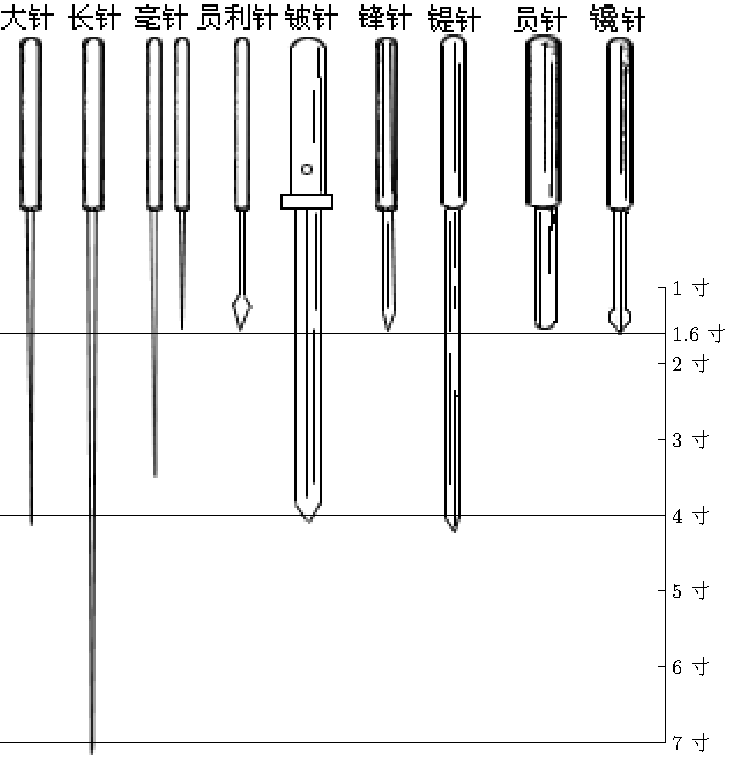
\includegraphics[width=0.50\textwidth]{九针图.pdf}\\
	\caption{九针图}\label{fig:九针图}
\end{figure}

\biaoti{【临证指要】}

\xiaobt{九针的应用}

九针,因其形状、长短等不同,在临床上的用途也各有不同。如《灵枢·官针》所说:“九针之宜,各有所为,长短大小,各有所施也。”《灵枢·刺节真邪》亦说:“刺痈者用铍针,刺大者用锋针,刺小者用圆利针,刺热者用镵针,刺寒者用毫针也。”现将《内经》所论概括如下:

(1)因病选针:病证有表里寒热虚实之异,则针有长短大小宽窄之殊。以表里深浅言,病在皮肤、分肉、脉络等表浅部位者,宜选用镵针、圆针和锋针;病在骨隙关节、脏腑等较深部位者,宜选用圆利针、长短和大针;病在皮肤、分肉,或病痹气痛不去者,因病情较轻而宜选用较小的圆针、毫针;病为大脓,或在五脏,或水肿不能过关节者,因病情较重而宜选用较大的铍针、锋针、大针。以寒热虚实言,表热轻浅,宜选用镵针、锋针;里热痈肿,宜选用锋针、铍针;正气不足者,宜选用𫔂针、圆针、毫针;邪气有余者,宜选用铍针、锋针、圆利针。

(2)因针施病:镵针:浅刺皮肤,可泻阳热邪气,主治头身之热。圆针:为按摩用针,能揩摩肌肉以泻分肉间的邪气,也可按压经络腧穴以疏通气血,还能用于放血、放水、放脓等方面。𫔂针:为按压穴位用针,能按压经脉腧穴通导气血,主治血脉病证;亦能用于探查痈脓部位深浅,开大疮口,疏通漏管的作用;因其还可扶正祛邪,故还能用于正气不足之证。锋针:能点刺放血以泻邪热,适用于血脉热瘀阻滞之顽证;还可挑破痈脓以放出脓血。铍针:为外科手术用具,可用于痈脓切排及其它手术。圆利针:用于需深刺的痈肿及暴痹。毫针:有通经络,散邪气,养正气的功用,常用于治疗寒热痛痹及邪浅在络等病证。长针:可用于治疗深部邪气及久痹。大针:主要用于利关节,泻积水。

\biaoti{【原文】}

\begin{yuanwen}
陽明多血多氣,太陽多血少氣,少陽多氣少血,太陰多血少氣,厥\sb{1}陰多血少氣,少\sb{2}陰多氣少血。故曰刺陽明出血氣,刺太陽出血惡氣,刺少陽出氣惡血,刺太陰出血惡氣,刺厥陰出血惡氣,刺少陰出氣惡血也。足陽明太陰爲表裏,少陽厥陰爲表裏,太陽少陰爲表裏,是謂足之陰陽也。手陽明太陰爲表裏,少陽心主爲表裏,太陽少陰爲表裏,是謂手之陰陽也。
\end{yuanwen}

\biaoti{【校注】}

\begin{jiaozhu}
	\item 厥:《灵枢·五音五味》作“少”,可从。
	\item 少:《灵枢·五音五味》作“厥”,可从。
\end{jiaozhu}

\biaoti{【理论阐释】}

\xiaobt{六经气血多少}

关于六经气血多少的论述,《内经》中凡三见:一见于本篇,二见于《灵枢·五音五味》,三见于《素问·血气形志篇》,但三篇所言之气血多少有异。(表\ref{tab:六经气血多少对照表})

\begin{table}[htb]%六经气血多少对照表
	\centering
	\caption{六经气血多少对照表}\label{tab:六经气血多少对照表}
	\begin{tabu}to.87\textwidth{X[-1.5c]*6{|X[c]}}
		\toprule
		\diagbox[height=2.5em]
		{篇名}{六经}& 太阳     & 少阳     & 阳明     & 少阴     & 厥阴     & 太阴     \\
		\midrule
		血气形志篇  & 多血少气 & 少血多气 & 多气多血 & 少血多气 & 多血少气 & 多气少血 \\ \hline
		五音五味    & 多血少气 & 多血少气 & 多血多气 & 多血少气 & 多气少血 & 多血少气 \\ \hline
		九针论      & 多血少气 & 少血多气 & 多血多气 & 少血多气 & 多血少气 & 多血少气 \\
		\bottomrule
	\end{tabu}
\end{table}

马莳认为,《灵枢》多误,当以《素问·血气形志篇》为正。但对六经气血多少之理,未予阐明。张志聪在注《素问·血气形志篇》中论述了此理,曰:“夫气为阳,血为阴,腑为阳,脏为阴,脏腑阴阳,雌雄相合,而气血之多少,自有常数。如太阳多血少气,则少阴少血多气;少阳少血多气,则厥阴多血少气。阳有余则阴不足,阴有余则阳不足,此天地盈虚之常数也。惟阳明则气血皆多,盖血气皆生于阳明也。”张氏之言,似亦有理,但仍有疏漏之处,即太阴气血多少尚未言及。以张氏之理推之,则太阴当为“少气少血”之经。若是,则与“脾胃者,仓廪之官,五味出焉”之旨不相符合。那么,太阴的气血究竟以多少为正?我们认为,脾胃合为“后天之本”、“气血生化之源”、太阴阳明的气血均应俱旺,才能满足机体生命活动的需要,因此,太阴之气血当为“常多血气”,或“常多血多气”。

考《太素》卷十任脉云:“太阳常多血少气,少阳常多气少血,阳明常多血少气,厥阴常多气少血,少阴常多血少气,太阴常多血少气。”杨上善注:“手足少阴、太阳多血少气,以阴多阳少也。手足厥阴、少阳多气少血,以阳多阴少也。手足太阴、阳明多血少气,以阴阳俱多谷气故也。”《太素》所载原文及杨上善之注,将太阴、阳明放在同等地位,均为“多血少气”,其立论有据,规律性强,说理充分,可以为信。

\biaoti{【临证指要】}

\xiaobt{六经气血多少理论的临床意义}

《内经》对六经气血多少的论述,反映了脏腑及其经脉的生理功能特点,对于临床具有重要指导意义。其一,指导治则治法的确立。经脉气血多少,乃脏腑精气多少的反映,因此在脏腑治疗用药时,应考虑其经脉气血多少的因素,如少气少血者,其气血易伤,治当兼顾气血之不足的生理特点。针刺方面更是如此,如太阳、厥阴为多血少气之经,针刺宜出血,忌出气;少阳、少阴为少血多气之经,针刺宜出气,忌出血;阳明、太阴为多气多血之经,针刺宜出血气。其二,指导针刺浅深及手法补泻。针刺浅深及补泻手法的运用与经脉的阴阳属性及气血多少有一定关系。根据《灵枢·经水》、《甲乙经·十二经水》等所载,其针刺浅深及留针时间,三阳经依次为少阳四分、五呼;太阳五分、七呼;阳明六分、十呼。三阴经依次为:厥阴一分、一呼或二呼;少阴二分、三呼;太阴三分、四呼。说明从总体上来看,三阳经的针刺深度和留针时间均多于三阴经。从阴、阳经分类来看,其针刺浅深和留针时间是,三阳经中,阳气多者多于阳气少者;三阴经中,阴气多者多于阴气少者。以上均可作为临床施针的参考。

\section{靈樞·血絡論}%第四節

\biaoti{【原文】}

\begin{yuanwen}
黃帝曰;願聞其奇邪而不在經者\sb{1}。岐伯曰:血絡\sb{2}是也。黃帝曰:刺血絡而仆\sb{3}者何也?血出而射\sb{4}者何也?血少黑而濁者\sb{5}何也?血出清而半爲汁\sb{6}者何也?發鍼而腫\sb{7}者何也?血出若多若少而面色蒼蒼\sb{8}者何也?發鍼而

面色不變而煩悗\sb{9}者何也?多出血而不動搖者何也?願聞其故。岐伯曰:脈氣盛而血虛者,刺之則脫氣,脫氣則仆\sb{10}。血氣俱盛而陰氣多者,其血滑,刺之則射\sb{11};陽氣畜積,久留而不瀉者,其血黑以濁,故不能射\sb{12}。新飲而液參於絡,而未合和於血也,故血出而汁別焉\sb{13};其不新飲者,身中有水,久則爲腫\sb{14}。陰氣積於陽,其氣因於絡,故刺之血未出而氣先行,故腫\sb{15}。陰陽之氣\sb{16},其新相得而未和合,因而瀉之,則陰陽俱脫,表裏相離\sb{17},故脫色而\sb{18}蒼蒼然。刺之血出多,色不變而煩悗者,刺絡而虛經,虛經之屬於陰者,陰脫故煩悗\sb{19}。陰陽相得而合爲痹者\sb{20},此爲內溢於經,外注於絡,如是者陰陽俱有餘,雖多出血而弗能虛也\sb{21}。

黃帝曰:相\sb{22}之奈何?岐伯曰:血脈者,盛堅横以赤,上下無常處\sb{23},小者如鍼,大者如筋,則而瀉之萬全也,故無失數\sb{24}矣。失數而反,各如其度\sb{25}。黃帝曰:鍼入而肉著\sb{26}者何也?岐伯曰:熱氣因於鍼則鍼熱,熱則肉著於鍼,故堅焉\sb{27}。
\end{yuanwen}

\biaoti{【校注】}

\begin{jiaozhu}
	\item 奇邪不在经者:张介宾:“奇邪,即《缪刺论》所谓奇病也。在络不在经,行无常处,故曰奇邪”。“者”后,《甲乙经》有“何也”二字,义长,可据补。
	\item 血络:即皮肤浅表视而可见之络脉。此又指皮肤浅表层有瘀血阻滞之络脉。张志聪注:“血络者,外之络脉、孙脉,见于皮肤之间,血气有所留积,则失其外内出入之机。”
	\item 刺血络而仆:刺血络出血而致昏仆倒地。
	\item 血出而射:刺血络出血,其血向外喷射。
	\item 血少黑而浊:少,《甲乙经》作“出”。可据改。血出黑而浊,即刺血络所出之血,色黑而浓稠。
	\item 血出清而半为汁:刺血络后,血出清稀,一半是澄清的汁液。
	\item 发针而肿:出针之后,局部皮肤肿胀。
	\item 面色苍苍:苍苍后,《太素》、《甲乙经》均有“然”字,可从。面色苍苍然,即面色苍白。
	\item 烦悗:悗,音义同“闷”。烦闷,即心胸烦闷。
	\item 脉气盛而血虚,刺之则脱气,脱气则仆:张志聪注:“气虽盛而血则虚者,若泻其气,则阴阳俱脱,故为仆倒。”
	\item 血气俱盛而阴气多者,其血滑,刺之则射:意为血气俱盛而阴血尤旺者,其血行滑利,刺其络则有血喷射而出。张志聪注:“俱盛者,经脉内外之血气俱盛也”。
	\item 阳气畜积,久留而不泻者,其血黑以浊,故不能射:张介宾注:“阳气久留而不泻,则阳邪日盛,阴血日枯,故血气黑以浊,所出不多,不能射也”。
	\item 新饮而液渗于络,而未合和于血也,故血出而汁别焉:意为新饮入胃,水液渗于络中而未奉心化赤为血,仍以水液(津液)状态存在,故刺络出血时,可出现既见血出又见液出的情况。张介宾注:“新饮入胃,未及变化而渗入于络,故血汁相半也。”
	\item 身中有水,久则为肿:张志聪注:“血乃水谷之津液所化,若不新饮而出而为汁者,乃身中之水也。”
	\item 阴气积于阳,其气因于络,故刺之血未出而气先行,故肿:阳,指阳分之络脉。脏腑经脉之血气汇积于皮肤肌腠之络脉,其血气随络脉而变动,针刺络脉如果气已行而血未出,瘀积于皮肤,局部肌肤就会出现肿胀。
	\item 阴阳之气:此指经脉与络脉的营卫气血。
	\item 其新相得而未和合,因而泻之,则阴阳俱脱,表里相离:张介宾注:“言血气初调,营卫甫定也。当此之时,根本未固,而妄施以泻,则阴阳表里俱致脱离,而衰危之色故见于面也”。
	\item 而:《太素》作“面”,义明,可从。
	\item 刺络而虚经,虚经之属于阴者,阴脱故烦悗:张介宾注:“取血者,刺其络也。若出血过多,必虚及于经,经之属阴者,主脏,脏虚则阴脱,故为烦悗”。
	\item 阴阳相得而合为痹:表里之邪气相合而致经络气血痹阻。
	\item 内溢于经,外注于络,如是者阴阳俱有余,虽多出血而弗能虚也:经属阴,络属阳,邪气既向内溢于经脉,又向外注于络脉,致使经络中的邪气俱盛而有余。刺其血络,虽出血量多,但所泻多为邪气,故不会招致正气受损。
	\item 相:张介宾注:“相,视也。”
	\item 血脉者,盛坚横以赤,上下无常处:瘀积的络脉,其状盛满坚硬而色红紫,或在上或在下,其位不固定。
	\item 无失数:张韦聪注:“数者,血脉出入之度数。”无失数,不要违背血脉出入之度数,亦即不要违背刺络的法度。
	\item 失数则反,各如其度:马莳注:“若失其术数,而与法相反,则凡或汁或射等证,各如其度以相应矣。”
	\item 肉著:局部肌肉紧紧裹住针身而捻转拔出困难。
	\item 热气因于针则针热,热则肉著于针,故坚焉:张介宾注:“针入而热,肉必附之,故紧涩难转而坚不可拔也。”
\end{jiaozhu}

\biaoti{【理论阐释】}

1.刺络出血法的原理及作用

络脉内连经脏,外通组织器官,是脏腑经脉气血营养脏腑组织的桥梁和枢纽。因此,络道的畅通与否是能否完成这一重要功能的先决条件。故张志聪《黄帝内经灵枢集注·血络论》说:“血络者,外之络脉、孙络,见于皮肤之间·血气有所留积,则失其外内出入之机矣。”刺络出血法的作用,概括起来主要有以下两个方面。一是刺去邪瘀,疏通络道。邪瘀阻滞络中,则络血不能正常渗灌,从而病变丛生。用刺络出血法刺出其邪瘀以达到治疗目的。二是驱除络邪,防邪传经。络与经相通,共同构成了一个封闭式循环,若有形之邪阻滞络中,则“势不能出于络外,故经盛入络,络盛返经,留连不已”(喻昌《医门法律·络脉论》)。当此之时,唯有及时运用刺络出血法祛除络中邪瘀,才能使经络正常循环。故《素问·调经论》说:“帝曰:刺留血奈何?岐伯曰:视其血络,刺出其血,无令恶血得入于经,以成其疾。”

2.刺血络的反应及其原因:本篇将刺络后的反应概括为“刺血络而仆”、“血出而射”、“血出黑而浊”、“血出清而半为汁”、“发针而肿”、“血出若多若少而面色苍苍然”、“发针而面色不变而烦悗”、“多出血而不动摇”等八种。上述八种情况,又可区分为以下两大类反应:

(1)针刺局部反应:①局部出血。血气俱盛而络中血气充足、血行流利的,可见“血出而射”;阳热蓄积,瘀积过久,可见“血出黑而浊”;刚刚饮水,水津与血尚未和合,可见“血出清而半为汁”。此外,还有血出或多或少等情况。②局部肿胀。血气积于络脉,出针时气先行,血后行而郁闭于肌腠,则可见“发针而肿”。

(2)病人神色反应:①神昏仆倒。经络中气盛血虚,刺之气随血脱,可见“刺血络而仆”。②心胸烦闷。刺络出血多,致使经虚脏衰,心神失养,可见“烦悗”。③面色苍白。阴阳未调,气血不固,妄用刺络法而使阴阳俱脱,气血耗散,可见“脱色面苍苍然”。④神色正常。邪气盛满于经络之中,正气旺盛未衰,刺之虽出血多,但属于正气驱邪外出的反应,不会伤及正气,故“多出血而不动摇”,表现为神色正常。

出现上述反应的原因,与以下四个方面的因素有关:一是病人体质的强弱。如“刺而仆”,多因体弱气血亏虚所致。临床上常见的晕针现象,亦常与此有关。“血出而射”,多因体强气血旺盛,血行流利而致。二是疾病轻重、病程长短。如“血出黑而浊”,多病程长而病情较重;“血出清而半为汁”,若非新饮,则多为“身中有水”所致。三是饮食质量及时间。如“出血清而半为汁”,多因新饮、多饮所致。四是医生技术水平和医疗态度。如“刺络而仆”,“发针而面色不变而烦悗”、“发针而肿”等反应,均与医生的技术水平和医疗态度有一定关系。

\biaoti{【临证指要】}

\xiaobt{刺络出血法的适应证及刺血度数}

《素问·血气形志篇》说:“凡治病必先去其血,乃去其所苦,伺之所欲,然后泻有余,补不足。”王冰注:“先去其血,谓见血脉盛满独异于常者乃去之,不谓常刺则先去其血也”。说明应用刺血法必须严格把握其适应证,做到有的放矢,切不可滥用。

依据《内经》所说,其刺络的适应证是血络有邪瘀阻滞,其表现是血络部可见“盛坚横以赤”、“小者如针,大者如筋”,亦即王冰所谓“血脉盛满独异于常者”。据此而刺,则攻邪而不伤正,所谓“则而泻之万全也”。因血络积聚程度的不同,刺络又有刺“结络”和刺“盛络”的区别。“结络”为瘀血留积较久较甚,刺之以去瘀血。《素问·三部九候论》说:“上实下虚,切而从之,索其结络脉,刺出其血,以见通之”。《灵枢·阴阳二十五人》亦说:“其结络者,脉结血不和,决之乃行”。“盛络”为邪气初聚,瘀血留积较轻,刺之以去邪气。《灵枢·经脉》说:“故刺诸络脉者,……甚血者,虽无结,急取之,以泻其邪而出其血。”“甚血者,虽无结”,是指络脉虽粗实胀起异于正常,但其血聚不甚明显,乃病邪初聚,血结不甚所致,急刺出血以泻其邪气。故《灵枢·根结》说:“此所谓十二经者,盛络皆为取之也”。《灵枢·脉度》亦说:“盛而血者,疾诛之。”

刺血度数,《内经》提出以“必无留血”作为标准。要做到这一点,一是“盛络皆为取之”,勿使遗漏;二是“视其血络,尽出其血”,除邪务尽。所谓“尽出其血”,《素问·刺腰痛篇》认为是“血变而止”,“见赤血而已”。可见,血色由暗转红,乃邪气已出的标志之一。以上原则,仍为今天临床所遵循。此外,还必须指出,临床上其刺血量的多少,还往往与病情轻重及所刺部位有关。故《内经》中还有“肺热病者,……刺手太阴、阳明,出血如大豆立已”,以及“顑痛,刺足阳明曲同动脉见血,立已”等记载,体现《内经》的原则性和灵活性。

\xiaojie

本章选编了《灵枢》和《素问》的四篇(段)原文,介绍了经络学说的主要内容。

十二经脉,即手足三阴三阳经,是经络的主要组成部分。其循行规律是:手三阴经,从胸走手,属脏络腑;手三阳经,从手走头,属腑络脏;足三阳经,以头走足,属腑络脏;足三阴经,从足走腹,属脏络腑。十二经首尾相贯,如环无端。十二经脉的病变包括经脉本身的病变及所联属脏腑的病变两大部分,所谓“是动病”,即经气变动而主要表现为经脉方面的病证,“所生病”,则为经气变动而主要表现为脏腑方面的病证。由于经脉内通脏腑,外连肢节,所以其病变表现的重心有经脉与脏腑的不同。

奇经八脉,包栝冲脉、任脉、督脉、带脉、阴跷、阳跷、阴维、阳维。奇经不与脏腑相通,交叉贯穿于十二经之间,具有加强经脉联系,调节各经气血阴阳的作用。其病变多表现在本经循行的部位上,如任脉为病,“男子内结七疝,女子带下瘕聚”;冲脉为病,“逆气里急”;督脉为病,“脊强反折”等。

络脉是经脉的补充,它主要分布在经脉所不到的部位,内至脏腑,外达体表,无处不到,是脏腑经络气血营养机体的桥梁与枢纽,在人体处于一个十分独特而又重要的地位。十五别络中,其十二经别络均起于四肢络穴,并联系其相表里的经脉;任脉之别散于腹;督脉之别散于头,别走足太阳经;脾之大络散布于前后胁肋。孙络的分布更为广泛,它们自大络别出后,越分越多,愈分愈细,分别弥散于经脉所属的内外区域内。

此外,本篇还讨论了六经气血多少及针刺宜忌;刺络出血法的适应证,刺血络的反应及其原因;九针的起源、命名、形状及其主治、禁忌;治疗风病、水病的俞穴;灸寒热病的取穴及方法等内容。

\zuozhe{(邱幸凡)}
\ifx \allfiles \undefined
\end{document}
\fi